% % arara: xelatex
% % arara: xelatex
% % arara: xelatex


% % options:
% % thesis=B bachelor's thesis
% % thesis=M master's thesis
% % czech thesis in Czech language
% % english thesis in English language
% % hidelinks remove colour boxes around hyperlinks

% \documentclass[thesis=B,english]{FITtemplates/FITthesis}[2019/12/23]

% %\usepackage[utf8]{inputenc} % LaTeX source encoded as UTF-8
% % \usepackage[latin2]{inputenc} % LaTeX source encoded as ISO-8859-2
% % \usepackage[cp1250]{inputenc} % LaTeX source encoded as Windows-1250

% % \usepackage{subfig} %subfigures
% % \usepackage{amsmath} %advanced maths
% % \usepackage{amssymb} %additional math symbols

% \usepackage{dirtree} %directory tree visualisation

% % % list of acronyms
% % \usepackage[acronym,nonumberlist,toc,numberedsection=autolabel]{glossaries}
% % \iflanguage{czech}{\renewcommand*{\acronymname}{Seznam pou{\v z}it{\' y}ch zkratek}}{}
% % \makeglossaries

% % % % % % % % % % % % % % % % % % % % % % % % % % % % % % % 
% % EDIT THIS
% % % % % % % % % % % % % % % % % % % % % % % % % % % % % % % 

% \department{Department of Applied Mathematics}
% \title{Autonomous car chasing}
% \authorGN{Pavel} %author's given name/names
% \authorFN{Jahoda} %author's surname
% \author{Pavel Jahoda} %author's name without academic degrees
% \authorWithDegrees{Pavel Jahoda} %author's name with academic degrees
% \supervisor{Ing. Jan Čech, Ph.D.}
% \acknowledgements{THANKS (remove entirely in case you do not with to thank anyone)}
% \abstractEN{Summarize the contents and contribution of your work in a few sentences in English language.}
% \abstractCS{V n{\v e}kolika v{\v e}t{\' a}ch shr{\v n}te obsah a p{\v r}{\' i}nos t{\' e}to pr{\' a}ce v {\v c}esk{\' e}m jazyce.}
% \placeForDeclarationOfAuthenticity{Prague}
% \keywordsCS{Replace with comma-separated list of keywords in Czech.}
% \keywordsEN{Replace with comma-separated list of keywords in English.}
% \declarationOfAuthenticityOption{1} %select as appropriate, according to the desired license (integer 1-6)
% % \website{http://site.example/thesis} %optional thesis URL


% \begin{document}

% % \newacronym{CVUT}{{\v C}VUT}{{\v C}esk{\' e} vysok{\' e} u{\v c}en{\' i} technick{\' e} v Praze}
% % \newacronym{FIT}{FIT}{Fakulta informa{\v c}n{\' i}ch technologi{\' i}}

% \setsecnumdepth{part}
% \chapter{Introduction}



% \setsecnumdepth{all}
% \chapter{State-of-the-art}

% \chapter{Analysis and design}

% Přidáme odstavec Text --- zejména ten odborný --- je nutné členit na odstavce. Každý odstavec by se měl týkat jednoho tématu, myšlenky\dots{} Odstavce od sebe musí být vizuálně oddělené. K tomu existuje několik vhodných stylů, které si popíšeme v jedné z následujících kapitol. Odstavce mohou být různě vysázené. V odborných textech je běžná sazba "do bloku". Při ní je nutné vhodně měnit mezislovní mezery. Jejich doporučená velikost je 0,25--0.33 čtverčíku.

% Požadavky jsou těchto typů:

% \chapter{Realisation}

% \setsecnumdepth{part}
% \chapter{Conclusion}


% \bibliographystyle{iso690}
% \bibliography{mybibliographyfile}

% \setsecnumdepth{all}
% \appendix

% \chapter{Acronyms}
% % \printglossaries
% \begin{description}
% 	\item[GUI] Graphical user interface
% 	\item[XML] Extensible markup language
% \end{description}


% \chapter{Contents of enclosed CD}

% %change appropriately

% \begin{figure}
% 	\dirtree{%
% 		.1 readme.txt\DTcomment{the file with CD contents description}.
% 		.1 exe\DTcomment{the directory with executables}.
% 		.1 src\DTcomment{the directory of source codes}.
% 		.2 wbdcm\DTcomment{implementation sources}.
% 		.2 thesis\DTcomment{the directory of \LaTeX{} source codes of the thesis}.
% 		.1 text\DTcomment{the thesis text directory}.
% 		.2 thesis.pdf\DTcomment{the thesis text in PDF format}.
% 		.2 thesis.ps\DTcomment{the thesis text in PS format}.
% 	}
% \end{figure}

% \end{document}

% TODO the distance and the angle vs the distance and angle




\documentclass{ctuthesis/ctuthesis}
\usepackage{subfig}
\usepackage{amsfonts}

\ctusetup{
	xdoctype = B,
	xfaculty = F8,
	mainlanguage = english,
	titlelanguage = english,
	title-english = {Autonomous Car Chasing},
	%title-czech = {Automaticke pronasledovani auta},
	department-english = {Department of Applied Mathematics},
	author = {Pavel Jahoda},
	supervisor = {Ing. Jan Čech, Ph.D.},
	supervisor-address = {Czech Technical University in Prague Faculty of Electrical Engineering  \\
	Center for Machine Perception},
	fieldofstudy-english = {Knowledge Engineering},
	keywords-czech = {samořídíci auto, RC auto, víceúlohové učení, autonomní řízení, hluboké učení, CARLA, simulace},
	keywords-english = {self-driving car, RC car, multi-task learning, autonomous driving, deep learning, CARLA, simulation},
	month = 5,
	year = 2020,
}

\ctuprocess

\begin{abstract-english}

Safe autonomous driving system must have fast reaction times to ultimately prevent accidents and crashes. A car chase is a situation that requires such fast reaction times.


In our work, we introduce a novel dual-task convolutional neural network capable of simultaneously performing object detection as well as coarsened semantic segmentation. Furthermore, we have developed an autonomous driving system that uses the dual-task neural network. The system has been integrated into a subscale vehicle platform attached to a high-speed RC car and has been evaluated by autonomously chasing another vehicle. The system architecture and results of the evaluation are presented. 

\end{abstract-english}



\begin{abstract-czech}
Bezpečné autonomní řízení musí mít rychlé reakce, aby bylo možné předejít nehodám a srážkám. Pronásledování auta je situace, která vyžaduje tyto rychlé reakce.


V naší práci představujeme novou víceúlohovou konvoluční neuronovou síť schopnou současně detekovat objekty a hrubě semánticky segmentovat obrázky. Dále jsme vytvořili autonomní řídící systém, který tuto víceúlohovou neuronovou síť využívá. Tento systém byl integrován do do platformy nazvané "subscale vehicle platform" připevněné na velmi rychlé RC auto na kterém byl následné systém testován pronásledováním dalšího vozidla. V této práci je prezentována achitektura systému a výsledky evaluace.
\end{abstract-czech}

% Acknowledgements / Podekovani
\begin{thanks}
I would like to express my deep gratitude to my supervisor Assistant Professor Ing. Jan Čech, Ph.D. for his patient guidance and willingness to devote his time to this work. I would also like to thank ToMi team (Michal Bahník, Dominik Filyo, Martin Vlašimský, and others) who have assembled the 1:5 RC car platform used as the self-driving chasing car. Furthermore, I would like to thank doc. Ing. Martin Hromčík, Ph.D. for lending me his 1:10 RC car that was used as the chased car.\par


Finally, I would like to extend my thanks to my parents for their support throughout my education and to my girlfriend Vanda for her support and for helping me film a promotional video of the autonomous car chase.
\end{thanks}

% Declaration / Prohlaseni
\begin{declaration}
		I hereby declare that the presented thesis is my own work and that I have cited all sources of information in accordance with the Guideline for adhering to ethical principles when elaborating an academic final thesis.
		
		I acknowledge that my thesis is subject to the rights and obligations stipulated by the Act No.\,121/2000~Coll., the Copyright Act, as amended. In accordance with Article~46~(6) of the Act, I hereby grant a nonexclusive authorization (license) to utilize this thesis, including any and all computer programs incorporated therein or attached thereto and all corresponding documentation (hereinafter collectively referred to as the ``Work''), to any and all persons that wish to utilize the Work. Such persons are entitled to use the Work in any way (including for-profit purposes) that does not detract from its value. This authorization is not limited in terms of time, location and quantity.
\end{declaration}



\begin{document}

\maketitle

\chapter{Introduction}
An autonomous car driving system capable of making fast and accurate decisions is important for making car transportation a safer activity. The reaction times of the system (especially in high speeds) have an impact on the human trust and acceptance of automated vehicles. The key aspects of driving autonomously include detecting other cars and interacting with them on the road. In this paper, we focus on testing a semi-autonomous system in these aspects by using a car chasing scenario. \par


A similar scenario -- car-following -- has been studied for more than half a century. Car-following models describe how drivers should follow each other in traffic stream. Oftentimes these theoretical models assume having precise data such as speed, distance, and acceleration at every time-stamp \cite{car_following}. However, with the advancements of machine learning and computer vision more practical car-following models have been developed and tested. These models use sensors such as LIDAR and camera to estimate the distance between the two cars \cite{lidar_highway}. The estimated information is then used to maintain a safe distance between the two cars while following the trajectory of the front car. The car-following models have been however typically tested in scenarios that didn't involve high speeds and sudden significant speed changes. \par
 
 
On the other hand, a car chase -- a vehicular hot pursuit of suspects by law enforcers -- typically involves high speeds and therefore fast reactions are necessary. In our scenario, a vehicle being pursued is driven by a person, while the vehicle that's chasing it is being controlled by an artificial intelligence-based system. The system architecture is similar to the DARPA Urban Challenge vehicles \cite{Bertha}\cite{darpa2}\cite{darpa_book} and consists of three parts: perception and localization, trajectory planning and a trajectory controller. \par


The thesis has the following structure. First, a theoretical background of the chasing algorithm is outlined. This includes related work and also a description of each part of the system. Then, an experiment section follows. The section includes testing in CARLA -- an open-source simulator for autonomous driving research \cite{CARLA}. Additionally, it has a real-world evaluation of the system deployed in a radio-controlled car (RC car for short). The real-world evaluation consists of an evaluation of a detector on a collected dataset and a practical chase in which the goal, similarly to the car-following model, is to maintain a determined distance between the two RC cars.




\chapter{Related work}




\chapter{Method}
\section{Overview}
\begin{figure}[]
    \centering
    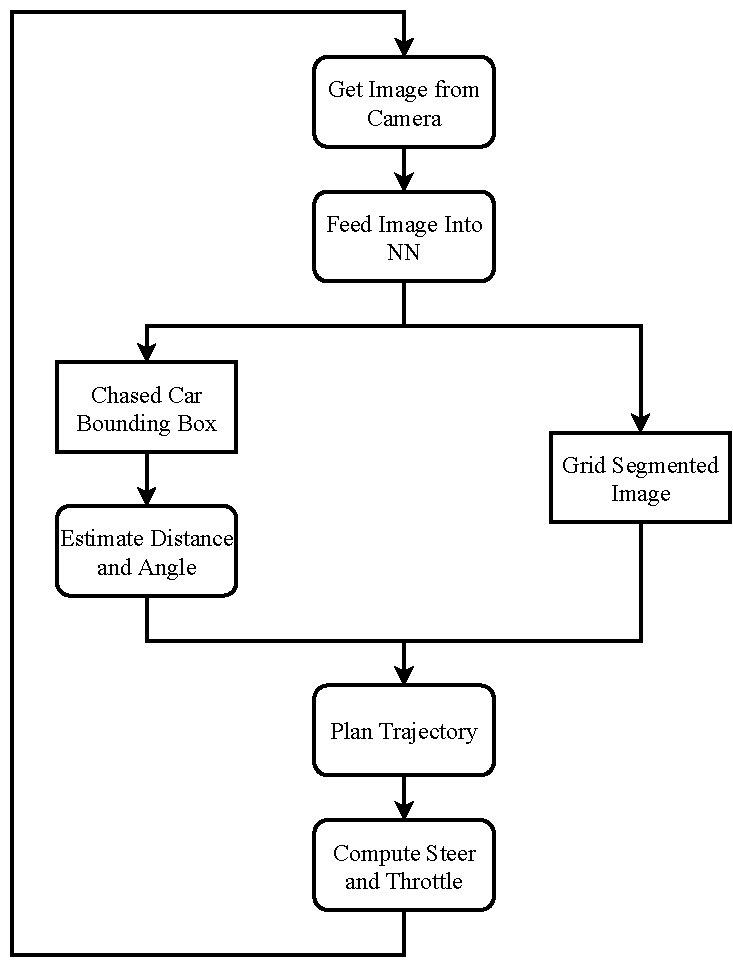
\includegraphics[width=0.7\textwidth]{images/bachelor_diagram.pdf}
    \caption{Simplified overview of the autonomous driving system}\label{f:overview}
\end{figure}

The system architecture is divided into three parts: perception and localization, trajectory planning and a trajectory controller. The architecture is depicted in the Figure \ref{f:overview}. \par


In the perception part, we introduce a novel neural network that detects objects and segments an image at the same time. It is able to find a 2D bounding box of the chased car. Furthermore, it segments an image into a coarsened grid of $S\times S$ cells and makes a classification about each cell whether it's drivable surface or not. The detection and segmentation are done with a single pass of the image through the neural network. \par


Then, we estimate the angle and distance between the two cars based on the detected bounding box of the chased car. In case no bounding box is found we extrapolate the distance and angle. \par


After the perception and localization, the trajectory is planned. At this stage, we take advantage of the image segmentation. If only drivable surface is between the two cars, we try to drive straight at the last position of the chased car. Otherwise, we use the image segmentation and find a direction where it's possible to drive and that is closest to the position of the chased car. \par


Finally, with the trajectory planned, we calculate the steer and throttle to drive the vehicle. We use a PID controller \cite{PID_orig} to control the throttle. It takes into account the current as well as the previous distances between the chasing and chased car. A Pure Pursuit \cite{pure_pursuit_orig} inspired algorithm is developed to control the steering. \par

Details of the method will be described in the following sections.




\section{Computer vision}
\subsection{Dual-task Neural Network}
In this section, we introduce a novel neural network that solves two problems at once - object detection and semantic segmentation. \par


The neural network shares the same backbone for both tasks -- a 53 layer feature extractor called Darknet-53 \cite{YOLOv3}. Attached to the feature extractor are two sets of layers -- one that gives the output for the object detection and the second that gives an output for the image segmentation. \par


The network is trained by alternating optimization. The neural network uses different loss functions depending on the batch. During training, when the network receives training batch of data for semantic segmentation, the output for the object detection is ignored and consequently only the shared layer and the segmentation layers are trained. Equivalently, when the network gets a batch containing object detection data, it updates the weights only on the shared layers and the detection layers. \par


During inference, the network works as follows. It is given an image, which passes through the network just once. From this, we get an object detection output as well as the semantic segmentation output. This means that while the training is slightly slower than training a single-task neural network, the extra cost is negligible during inference since the backbone features are shared. \par


For autonomous driving, the neural network architecture has many advantages over using two separate networks. First, as was mentioned, it is much faster. That is crucial when driving autonomously because we want to process as many frames per second as possible and have fast reaction times to ultimately prevent accidents and crashes. Second, it uses less memory, because most of the network weights are shared. This is potentially beneficial for the overall speed since more RAM is available, less disk swapping is required. Finally, it makes integration of the detection and segmentation into our autonomous RC car system a lot simpler.




\subsection{Bounding Box Detector}
In our work, a bounding box is the smallest 2D axis-aligned rectangle that encloses all pixels belonging to the chased RC car in an image. The detection is performed by a convolutional neural network \cite{CNN_Lecun} with YOLOv3 neural network architecture \cite{YOLOv3}. \par 
The first version of the YOLO published in 2015 \cite{YOLO}, made a great improvement to the previous state-of-the-art object detection solutions with its ability to predict bounding boxes of multiple object classes with incredible inference speed. It works by reasoning globally about the whole images and all its object classes. \par


\begin{figure}[h!]
    \centering
    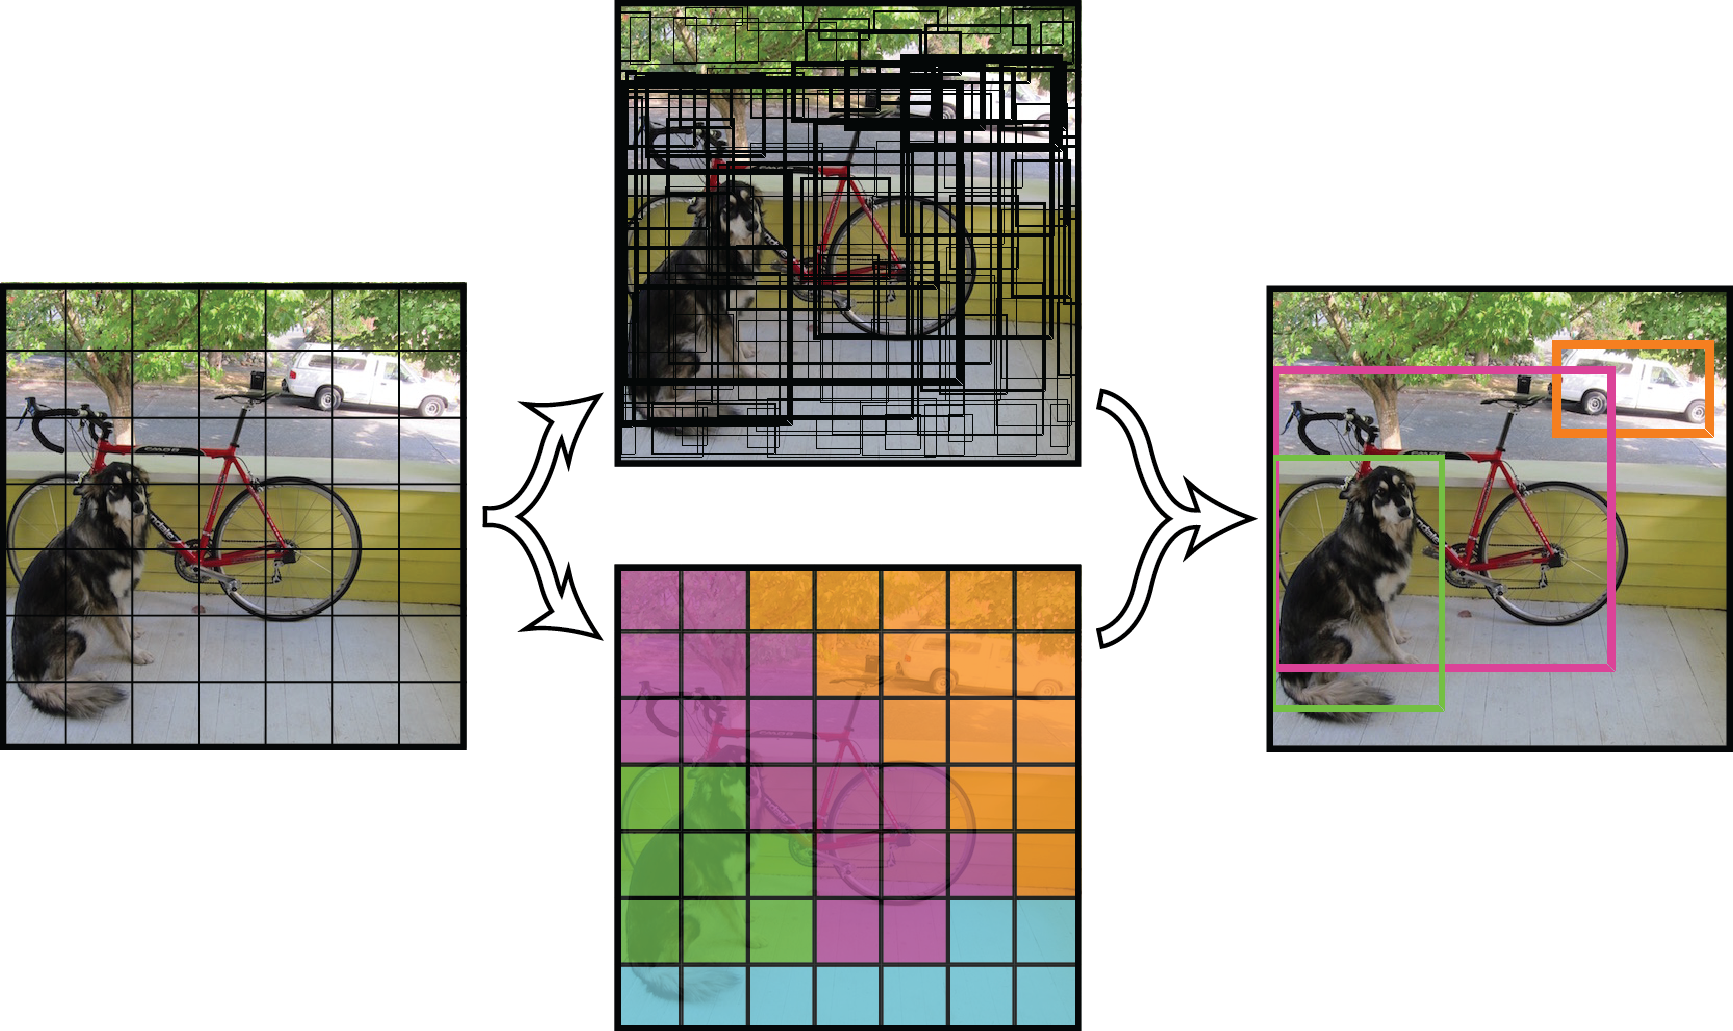
\includegraphics[width=0.8\textwidth]{images/YOLO.png}
    
    \caption{Diagram showing YOLO neural network mechanism, adopted from \protect\cite{YOLO}}\label{f:YOLO}
\end{figure}

The YOLO neural network divides an image into $S\times S$ grid of cells. Each cell makes $K$ bounding box predictions. Each prediction is a set of numbers such as width, height and the $(x,y)$ coordinates of the center of the bounding box. For each object in the image, the cell that has the center of the object inside is responsible for predicting its bounding box. This can be seen in the top middle image in the Figure \ref{f:YOLO}. Concurrently, each cell outputs $C$ values where each value represents a predicted probability of whether an object from a class $C_i$ is in the cell. The resulting class map from these predicted probabilities are seen in the bottom middle image in the Figure \ref{f:YOLO}. Both of these predictions -- the class probabilities and the bounding box predictions -- are then used together to make detection and classification of the objects in the image.
\par

During training, YOLO optimizes multi-task loss function. It concurrently optimizes the bounding box regression as well the class probabilities predictions.


Two years after introducing YOLO, the second version of called YOLO9000 \cite{YOLO9000} was introduced. In the first version of YOLO, each cell makes $K$ bounding box predictions of a random size. This was improved by calculating the expected bounding box sizes by clustering the bounding boxes of the training set. These expected bounding boxes are called anchors or priors. Furthermore, YOLO9000 also uses different network architecture called Darknet-19 and enables detection on different image sizes. \par


The third version of the YOLO architecture \cite{YOLOv3} improves YOLO in two main ways. Firstly, it adds more layers to the Darknet network architecture. Secondly, inspired by Feature Pyramid Networks \cite{FPN}, it predicts boxes at 3 different scales. To be specific, instead of dividing the image into $S\times S$ grid of cells, YOLOv3 divides it into $S\times S$, $(S\cdot2)\times (S\cdot2)$ and a $(S\cdot4)\times (S\cdot4)$ grid of cells. This helps the neural network to detect objects across a larger range of scales.


In our work, we have used the YOLOv3 detector pre-trained on a COCO dataset consisting of more than 330 000 images with objects from 80 different classes \cite{COCO_dataset}. The neural network was fine-tuned on our dataset that has 460 images of the chased RC car. The dataset is described in Section \ref{s:detection_dataset}. During fine-tuning, only the final layers that follow the Darknet-53 feature extractor were updated.




\subsection{Angle and Distance Estimation}
One of the most crucial information when chasing another vehicle is it's relative angle and distance to the chasing car as sketched in Figure \ref{f:chasing_diagram}. In our work, we are estimating the angle between the heading vector of the chasing car and the vector pointing from the center-front of the chasing car to the center of the back of the pursued car. Furthermore, we estimate the distance between the two cars. To be specific, the distance between $d$ the front of the chasing car and the center of the back of the pursued car. \par


\begin{figure}[h!]
    \centering
    \includegraphics[width=0.7\textwidth]{images/ChasingDiagram.png}
    
    \caption{Angle and distance estimation: Blue chasing car on the left and pursued car on the right. It shows the ground truth distance $d$ and the angle $\varphi$ we are estimating using camera mounted on the chasing car }\label{f:chasing_diagram}
\end{figure}

Figure \ref{f:chasing_diagram} shows this problem in a simplified 2D view. To estimate the distance and the angle of the car from an image, we took advantage of existing solutions solving PnP (Perspective-n-Point) problem. The PnP is a problem of estimating position and orientation of a camera from a set of $n$ known 3D points, their corresponding 2D projections in the image and the calibrated intrinsic camera parameters. This leads us to the following camera projection equation: \par


\begin{equation}
s\,\mathbf{p_{image}} = \mathbf{K}\,[\,\mathbf{R}\, |\, \mathbf{T}\, ]\, \mathbf{p_{model}}
\end{equation}

The $\mathbf{p_{image}}$ are the coordinates of the points in the image, $\mathbf{p_{model}}$ are the 3D model coordinates, $\mathbf{K}$ is the matrix of intrinsic camera parameters and $\mathbf{R}$ and $\mathbf{T}$ are the rotation and translation we are estimating. This can be further rewritten as: \par


\begin{equation}
s\begin{bmatrix}u\\v\\1\end{bmatrix} = \begin{bmatrix}
f_x & \gamma & u_0\\
0 & f_y & v_0\\
0 & 0 & 1
\end{bmatrix}\begin{bmatrix}
r_{11} & r_{12} & r_{13} & t_{1}\\
r_{21} & r_{22} & r_{23} & t_{2}\\
r_{31} & r_{32} & r_{33} & t_{3}\\
\end{bmatrix}
\begin{bmatrix}x\\y\\z\\1\end{bmatrix}
\end{equation}

In our case, the image points $p_{image}$ are the bounding box corners of the detected car. We also estimated the world coordinates $p_{world}$ by measuring the width and height of the chased RC car. Finally, the intrinsic camera parameters such as focal lengths $f_x$ and $f_y$ were taken from official calibration of the ZED camera. Then, we plugged these values into an OpenCV \cite{opencv_library} library function which gave us the translation and rotation vectors. Afterwards, we calculated the distance $d$ by calculating the Euclidean distance between the translation vector $\mathbf{T}$ and the origin. Similarly, we extracted the desired estimated angle $\varphi$ by calculating arc tangent of the rotation vector. 

Finally, since we are using a stereo camera and the camera lens which was used is not in the center of the front of the car, we converted the calculated angle and distance as if the camera was in the center of the front of the car. We achieve this by a simple triangulation.

\subsection{Angle and Distance Extrapolation}
In the previous section, we have described how we estimate angle distance based on the bounding box of the chased car. However, in some cases the detector is unable to detect the object in the image due to poor light conditions in the scene, or because the pursued vehicle is only partially visible due to some object occluding it. Furthermore, there are cases when the chased car is out of field of view. In these cases, we need to make a reasonable prediction about the position of the chased car. \par


We extrapolate the angle and the distance of the chased car based on the previous estimates. At the heart of the extrapolation algorithm is an exponential moving average. In fact, we use just six variables to store information about the whole history of estimated angles and distances. The idea will be explained on the process of extrapolating distances. The angle extrapolation is done similarly. \par


Every frame we update exponential moving average variable using following equation:\par


\begin{equation}
    \hat{e_{i}}=
    \begin{cases}
      \alpha\cdot d_i + (1-\alpha)\cdot \hat{e}_{i-1}, & \text{if bounding box found} \\
      \alpha\cdot d_{extrapolated} + (1-\alpha)\cdot \hat{e}_{i-1}, & \text{otherwise}
    \end{cases}
\end{equation}

Where $\hat{e_{i}}$ is the exponential moving average variable at $i$th frame, $\alpha$ is a value in the range [0,1] that sets the weight of the last predicted distance. In our algorithm, we have chosen value $\alpha=0.5$. \par

If the chased car is detected at $i$th frame, we set $d_i$ equal to the predicted estimate received from the PnP. We then update the variable $\hat{e_{i}}$ using the estimate $d_i$ and subsequently output the variable $d_i$ as our estimate for $i$th frame. In case no bounding box was detected, we update the $\hat{e_{i}}$ variable with $d_{extrapolated}$ variable that is computed using the following linear extrapolation equation:


\begin{equation}
d_{extrapolated} = 2\cdot d_{i-1} - d_{i-2}
\end{equation}

Afterwards, we output the variable $\hat{e_{i}}$ as our estimate for $i$th frame in case no bounding box was detected. Then, we set $d_i = d_{extrapolated}$ for future linear extrapolation computations. Finally, each extrapolated angle is processed by a saturation block that limits the output values. The saturation limits are -175 and 175 degrees. \par


This method allows us to extrapolate the angle and the distance very fast in a $\mathcal{O}(1)$ time and space complexity with almost no overhead.




\subsection{Image Segmentation}
In comparison to the semantic segmentation that links each pixel of the image to a class label, we segment the image into a coarsened grid of $S\times S$ cells. Each cell linked with a class label. In our work, we have chosen $S=10$ and only two classes. The first class represents a drivable surface while the second class is everything else. \par


\begin{figure}[h!]
    \centering
    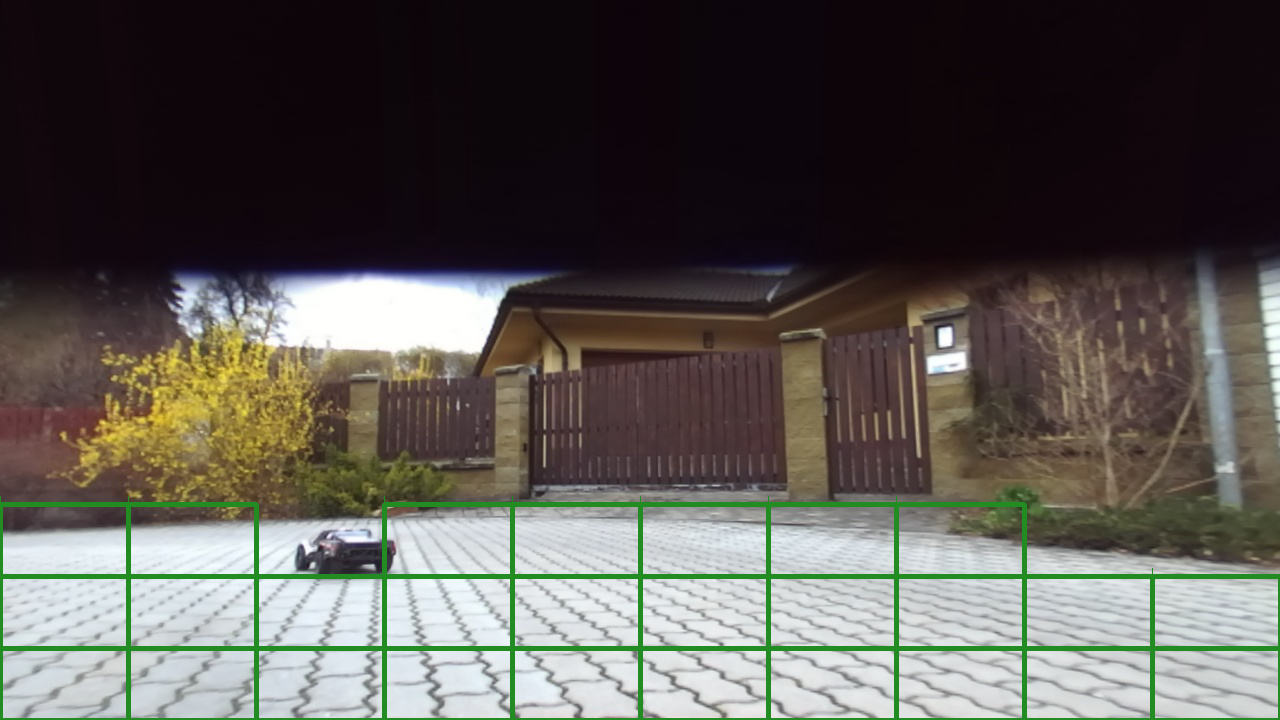
\includegraphics[width=0.8\textwidth]{images/segmented_image.png}
    
    \caption{Segmented image from the RC car's camera. The image is segmented into $10\times 10$ grid of cells where the green cells represent a drivable surface. The image is taken from our test set}\label{f:segmented_image}
\end{figure}

To create a labeled dataset, we used semantic segmented images (an image that has each pixel of the image linked to a class label). Then, we calculate the number of pixels in a cell that belong to the class representing the drivable surface. If the percentage of these pixels is higher than $P$ percentage of all the pixels in the cell, we assign the cell said label. In our work, we have chosen $P=50\%$.\par


Since we have only two classes we can represent each cell label as binary 1 or 0. For this reason, we have chosen the logistic loss function to train the network. \par

\begin{equation}
L_{log} = -\dfrac{1}{N} \sum_{i=1}^{N} y_i \cdot \log_{} (\hat{y_i}) + (1 - y_i) \cdot \log_{} (1-\hat{y_i})
\end{equation}

Where $N$ is the number of images per batch, $\hat{y_i}$ are the predicted segmentation values of the neural network for the $i$th image in the batch and $y_i$ are its labels. 




\section{Control And Planning}
In this section, we will explain how we control the steering and throttle of the vehicle based on the extracted information from the camera. Conversely to many algorithms \cite{Broggi2013}\cite{Werling2010}, we control steering and throttle separately. Steering control is inspired by pure pursuit algorithm and throttle is controlled by a PID controlled.


\subsection{Pure Pursuit Inspired Algorithm} \label{sec:pure_pursuit}
Pure pursuit algorithm is a path tracking algorithm that moves a vehicle from its current position to some look-ahead position on the path. It was invented in the 1980s as it was used in the first demonstration of an autonomous vehicle capable of following a road using imagery from a black and white camera \cite{pure_pursuit_orig}. The goal of the demonstration was to keep the vehicle centered on the road while it was driving at a constant speed.\par


The algorithm works as follows. Firstly, it finds the goal point on the path. Then, it transforms the goal point to vehicle coordinates and finally it calculates the curvature that will drive the vehicle to the look-ahead position on the path. \par


In our work, we were inspired by the algorithm. As opposed to the pure pursuit algorithm settings, our car doesn't move at a constant speed. Secondly, we are not following a path, but rather chasing a moving RC car. Therefore, every time we process an image from the camera, we update our goal position. But unlike in the path-following algorithm, the target position is updated with respect to the current position of the chased RC car rather than to a position on a path. \par
Conversely to the pure pursuit algorithm, we also do not calculate the curvature to control the steering. That is because we need to update the steering every frame based on the position of the chased RC car and take more aggressive turns to chase the pursued vehicle. In our algorithm we calculate the steering value with the following function:

\begin{equation}steer = (\cfrac{\alpha}{\textrm{180}})^{2}\end{equation}

Value $\alpha$ represents the angle between the chasing and the chased car shown in the Figure \ref{f:chasing_diagram}. The $steer$ variable is a value in the [-1, 1] range, where -1 and 1 represent the highest left-turn and right-turn steering angle the car can make respectively. We square the result of the division because the steering control on the RC car is non-linear. We don't square the division in the CARLA simulation.




\subsection{Semantic Segmentation Based Planning}
During inference, we use the coarsened segmented grid in the following way. First, we construct a line from the middle (horizontally) bottom (vertically) of the image to the bounding box of the detected car. If this line goes only through cells that are drivable, the trajectory planning phase stays unchanged and we try to follow the car directly as described in Section \ref{sec:pure_pursuit}. If that's not the case, we repeat the construction of the line. This time, however, the line goes from the middle bottom of the image to other cells on the same horizontal line as the bounding box of the car. When we find a line goes through cells with drivable surfaces and that is closest to the RC car, we try to drive the car in this direction until it's possible again to chase the car directly.

\subsection{PID Controller}
Despite being invented in the 1940s, the PID controller is the most common control algorithm. In a 2002 survey of over 11 000 controllers from various industries, it was found that 97\% of regulatory controllers utilize PID feedback \cite{PID-usage}. 

In our work, we use a PID controller to control the throttle of the chasing autonomous car. As the name suggests it can be described with the following equation:

\begin{equation}
throttle = P+I+D    
\end{equation}
The term $P$ called the proportional term is equal to a value proportional to the current error value $e_i$. In our case, the error value is $e_i = d_i - d_{desired}$, where $d_i$ is the estimated distance between the chasing and the chased car, and $d_{desired}$ is the desired distance between the two cars that we are trying to maintain. Equivalently to the terms $I$ and $D$, the term $P$ is equal to a value multiplied by a weight $w_p$ which indicates the influence and importance of the term. Therefore, the term $P$ is described as $P = e_i\cdot w_p$ \par


The term $I$ refers to the integration term. It integrates the errors over time. In our case, if the distance between the two cars continues to stay too large for a prolonged period, this term increases its value. It is equal to $I = w_i\cdot \sum_{j=(i-K)}^{i} e_j$, where K is the number of frames representing the time we want to consider from the current frame. We used $K = 300$, which corresponds to the last 10 seconds.\par


The last component of the equation -- $D$ refers to the derivation term. Its purpose is to decrease the rate of change and decrease oscillations of the error value. In our work $D = w_d\cdot (e_i-e_{i-1})$. \par


To make the PID controller usable based on the dynamics of the system, weights of the three components must be set. We have picked different weights for the CARLA simulation and the RC car. In the CARLA simulation, we have analyzed over a hundred sets of weights and picked the one that resulted in the lowest average error ($e = d - d_{desired}$). These values were $w_p=0.1$, $w_i=0$ and $w_d=1$. For the RC car, we have chosen the values based on trial and error. They were $w_p=0.25$, $w_i=0$ and $w_d=0.07$. Finally, we saturate the output to the [0, 1] range. \par


The reason for choosing $w_i=0$ is pretty simple. While higher value of $w_i$ had a positive effect on the average error, it caused the car to crash into the chased car. In many cases, if the car was not catching up it made the car drive very fast and when it reached the desired distance, the car didn't slow fast enough resulting in a crash. Lowering the number of frames the integration part considers, did slightly help this issue. However, we decided not to take the risk of breaking a very expensive subscale vehicle platform attached to the RC car.



\chapter{Experiments}

\section{Vehicle Detection}
\subsection{Dataset} \label{s:detection_dataset}
In order to train and evaluate 2D object detector capable of creating 2D bounding box around the chased RC car in a image, a dataset was needed. The collected dataset consists of \textbf{460} annotated images. All image annotations are in the PASCAL VOC data format introduced in the PASCAL Visual Object Classes Challenge \cite{pascal-voc}. Each image has it's annotation that contains pixel coordinates of the bounding box corners for each object in the image. In our dataset, only one object per image is present -- the chased RC car. The data were collected from multiple locations around Czechia and also under different lighting conditions. The majority of images were collected by the ZED Stereo camera attached to the chasing RC car. 

\begin{figure}[h!]
    \centering
    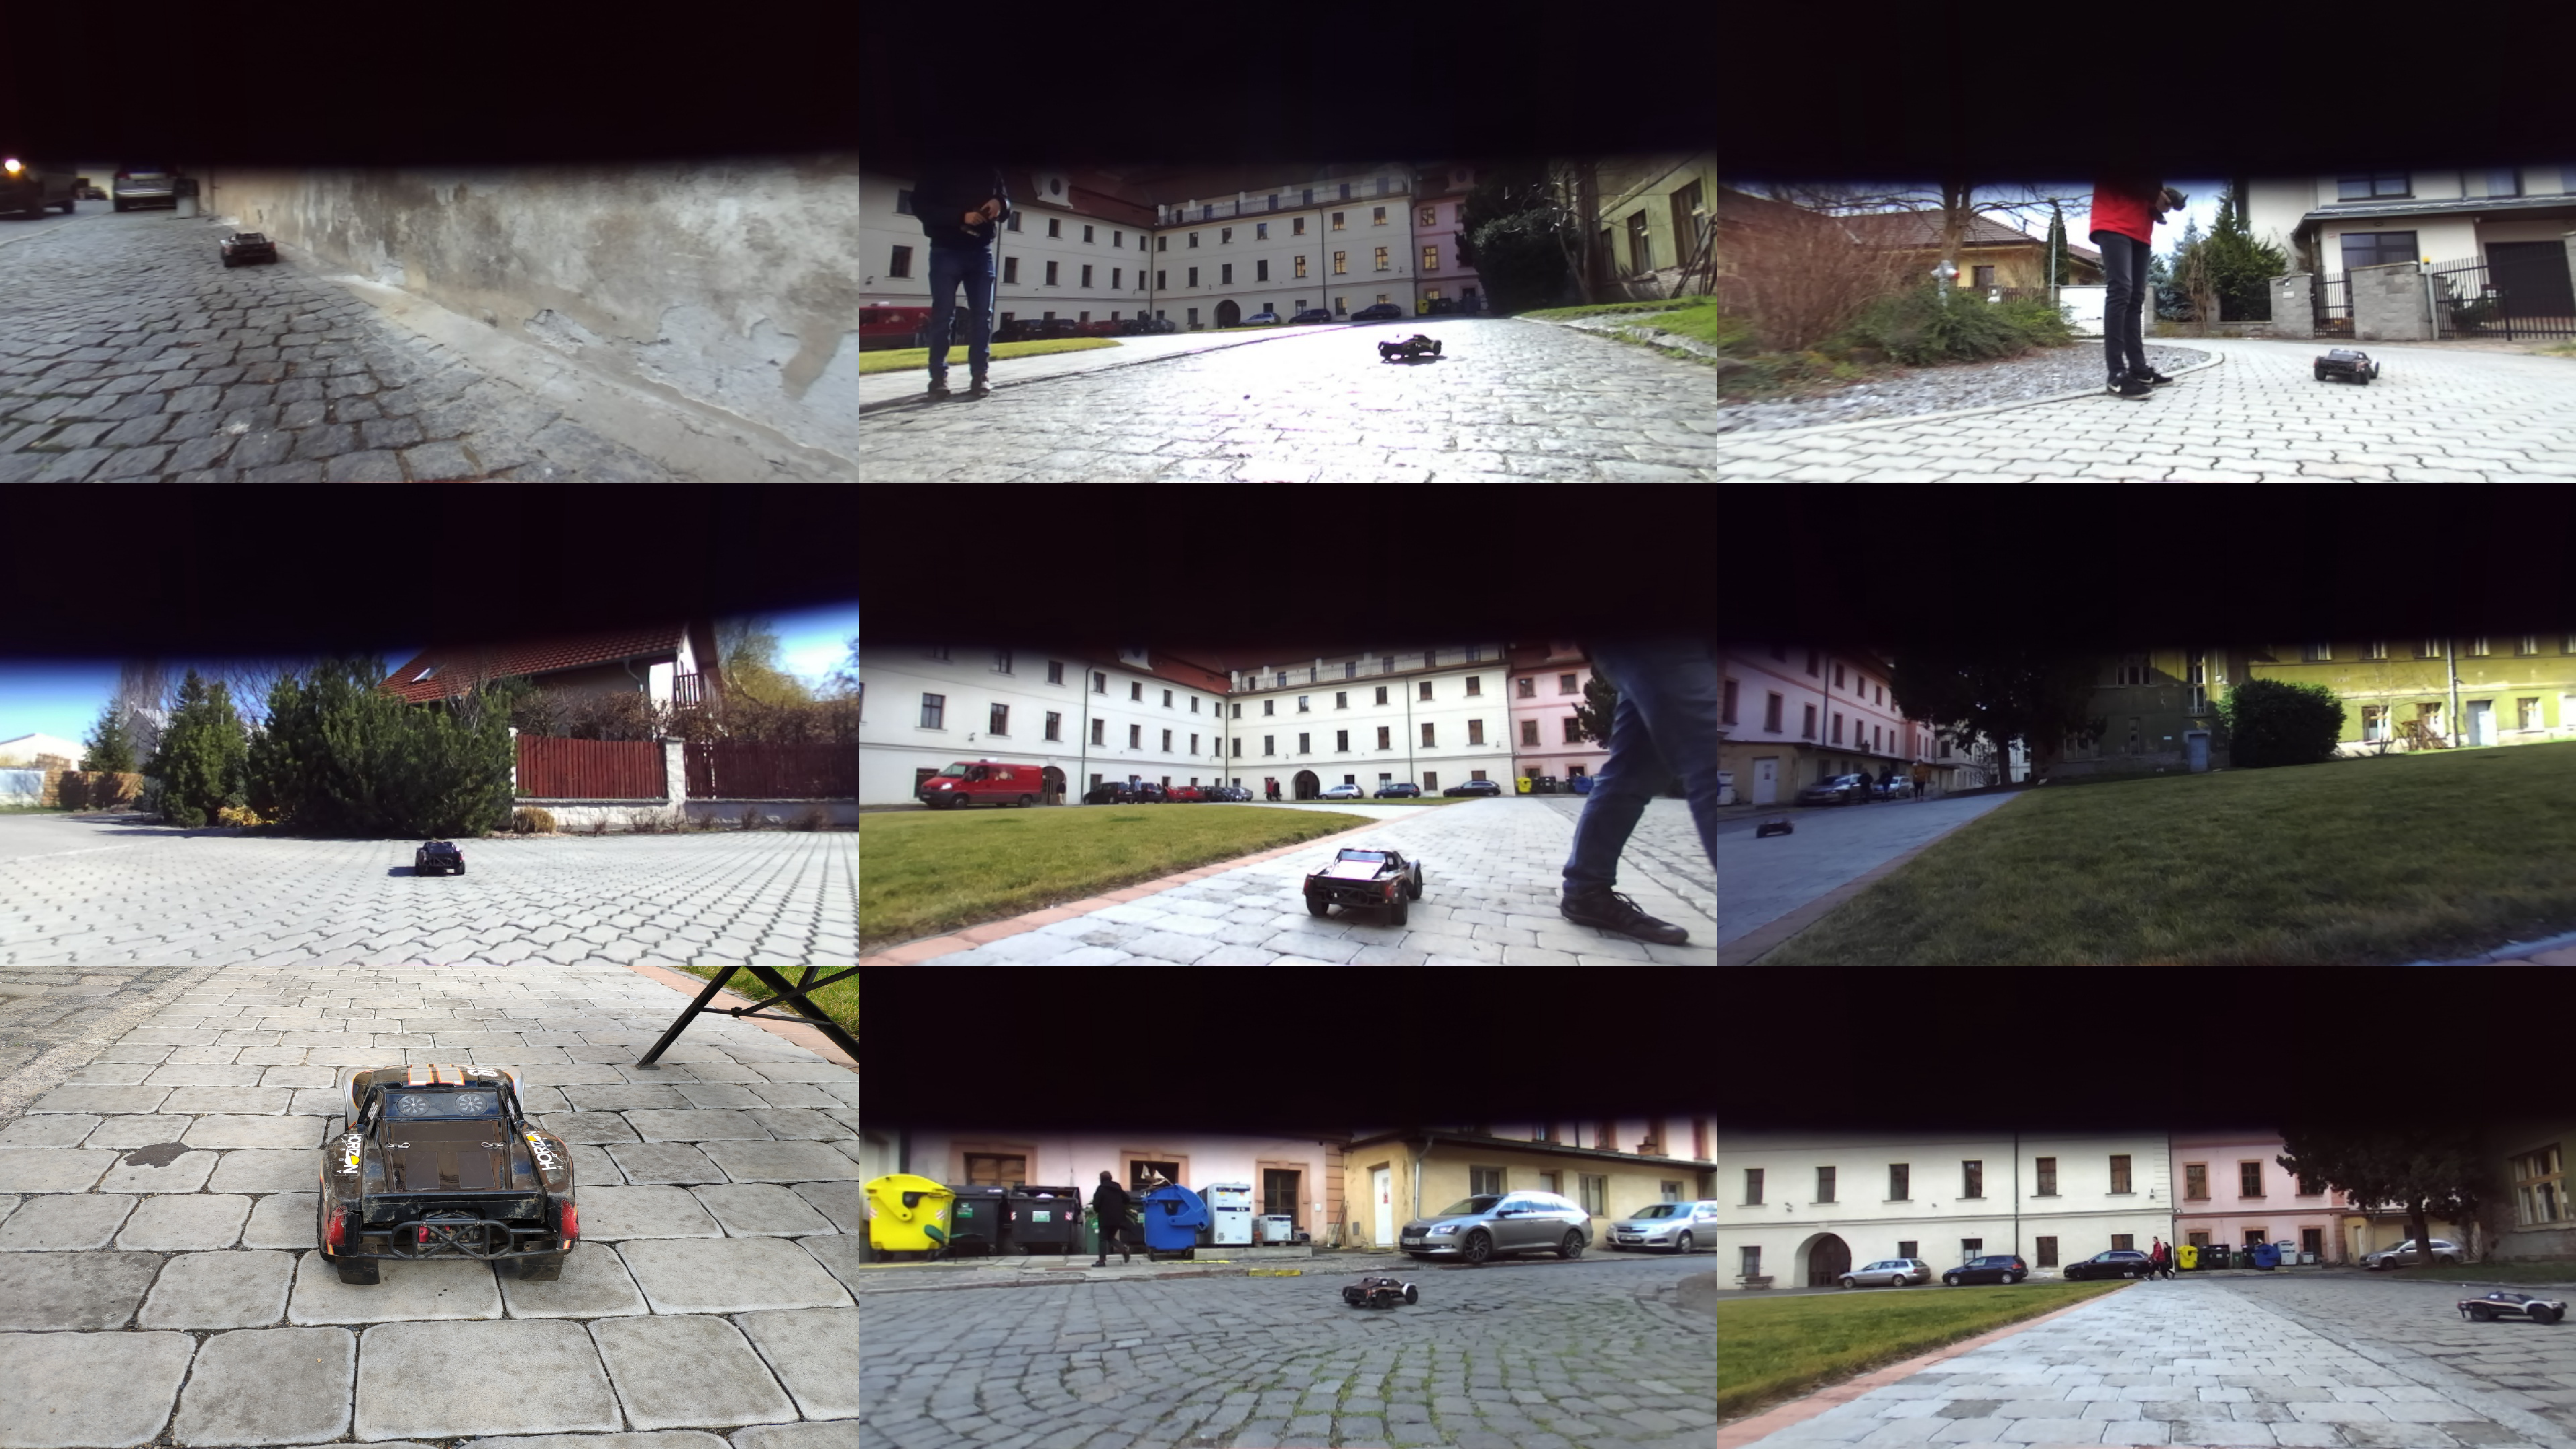
\includegraphics[width=1\textwidth]{images/dataset_collage.pdf}
    
    \caption{Detection dataset. Overview of the environment variability present in the dataset}\label{f:dataset_detection}
\end{figure}


\subsection{Detection Results}
The collected dataset was split into three sets. The majority of 80\% of the images were randomly selected into training set, 10\% were randomly selected into validation set and the remaining images were used as a test set. To evaluate the model, we calculated multiple values -- recall, precision, XY loss and WH loss. To understand recall and precision we need to first define IoU (Intersection over union). IoU measures how much the predicted bounding box overlaps with the ground truth (annotated bounding box). It is defines as 
\begin{equation}IoU = \cfrac{\textrm{Area of overlap}}{\textrm{Area of union}}\end{equation}

When calculating precision and recall, we say that the predicition is either true positive or false positive when IoU is bigger than $0.5$. XY loss is calculated as a mean squared error (MSE) between the center of the predicted bounding box and the center of ground truth bounding box. WH loss on the other hand is the difference between width and height of the predicted bounding box and the ground truth bounding box. When calculating both of these values, coordinates and image dimensions have been scaled to the [0, 1] range. \par
During training, the model with the lowest loss on the validation dataset has been saved.

\begin{table}[]
\begin{tabular}{l|llll}
\hline
            & Precision & Recall & XY loss & WH loss \\ \hline
Testing set & 99.8\%    & 97.7\% & 0.066   & 0.227   \\ \hline
\end{tabular}
\label{tab:detection}
\caption{Evaluation of the detector on a testing set}
\end{table}



\begin{figure}[h!]
    \centering
    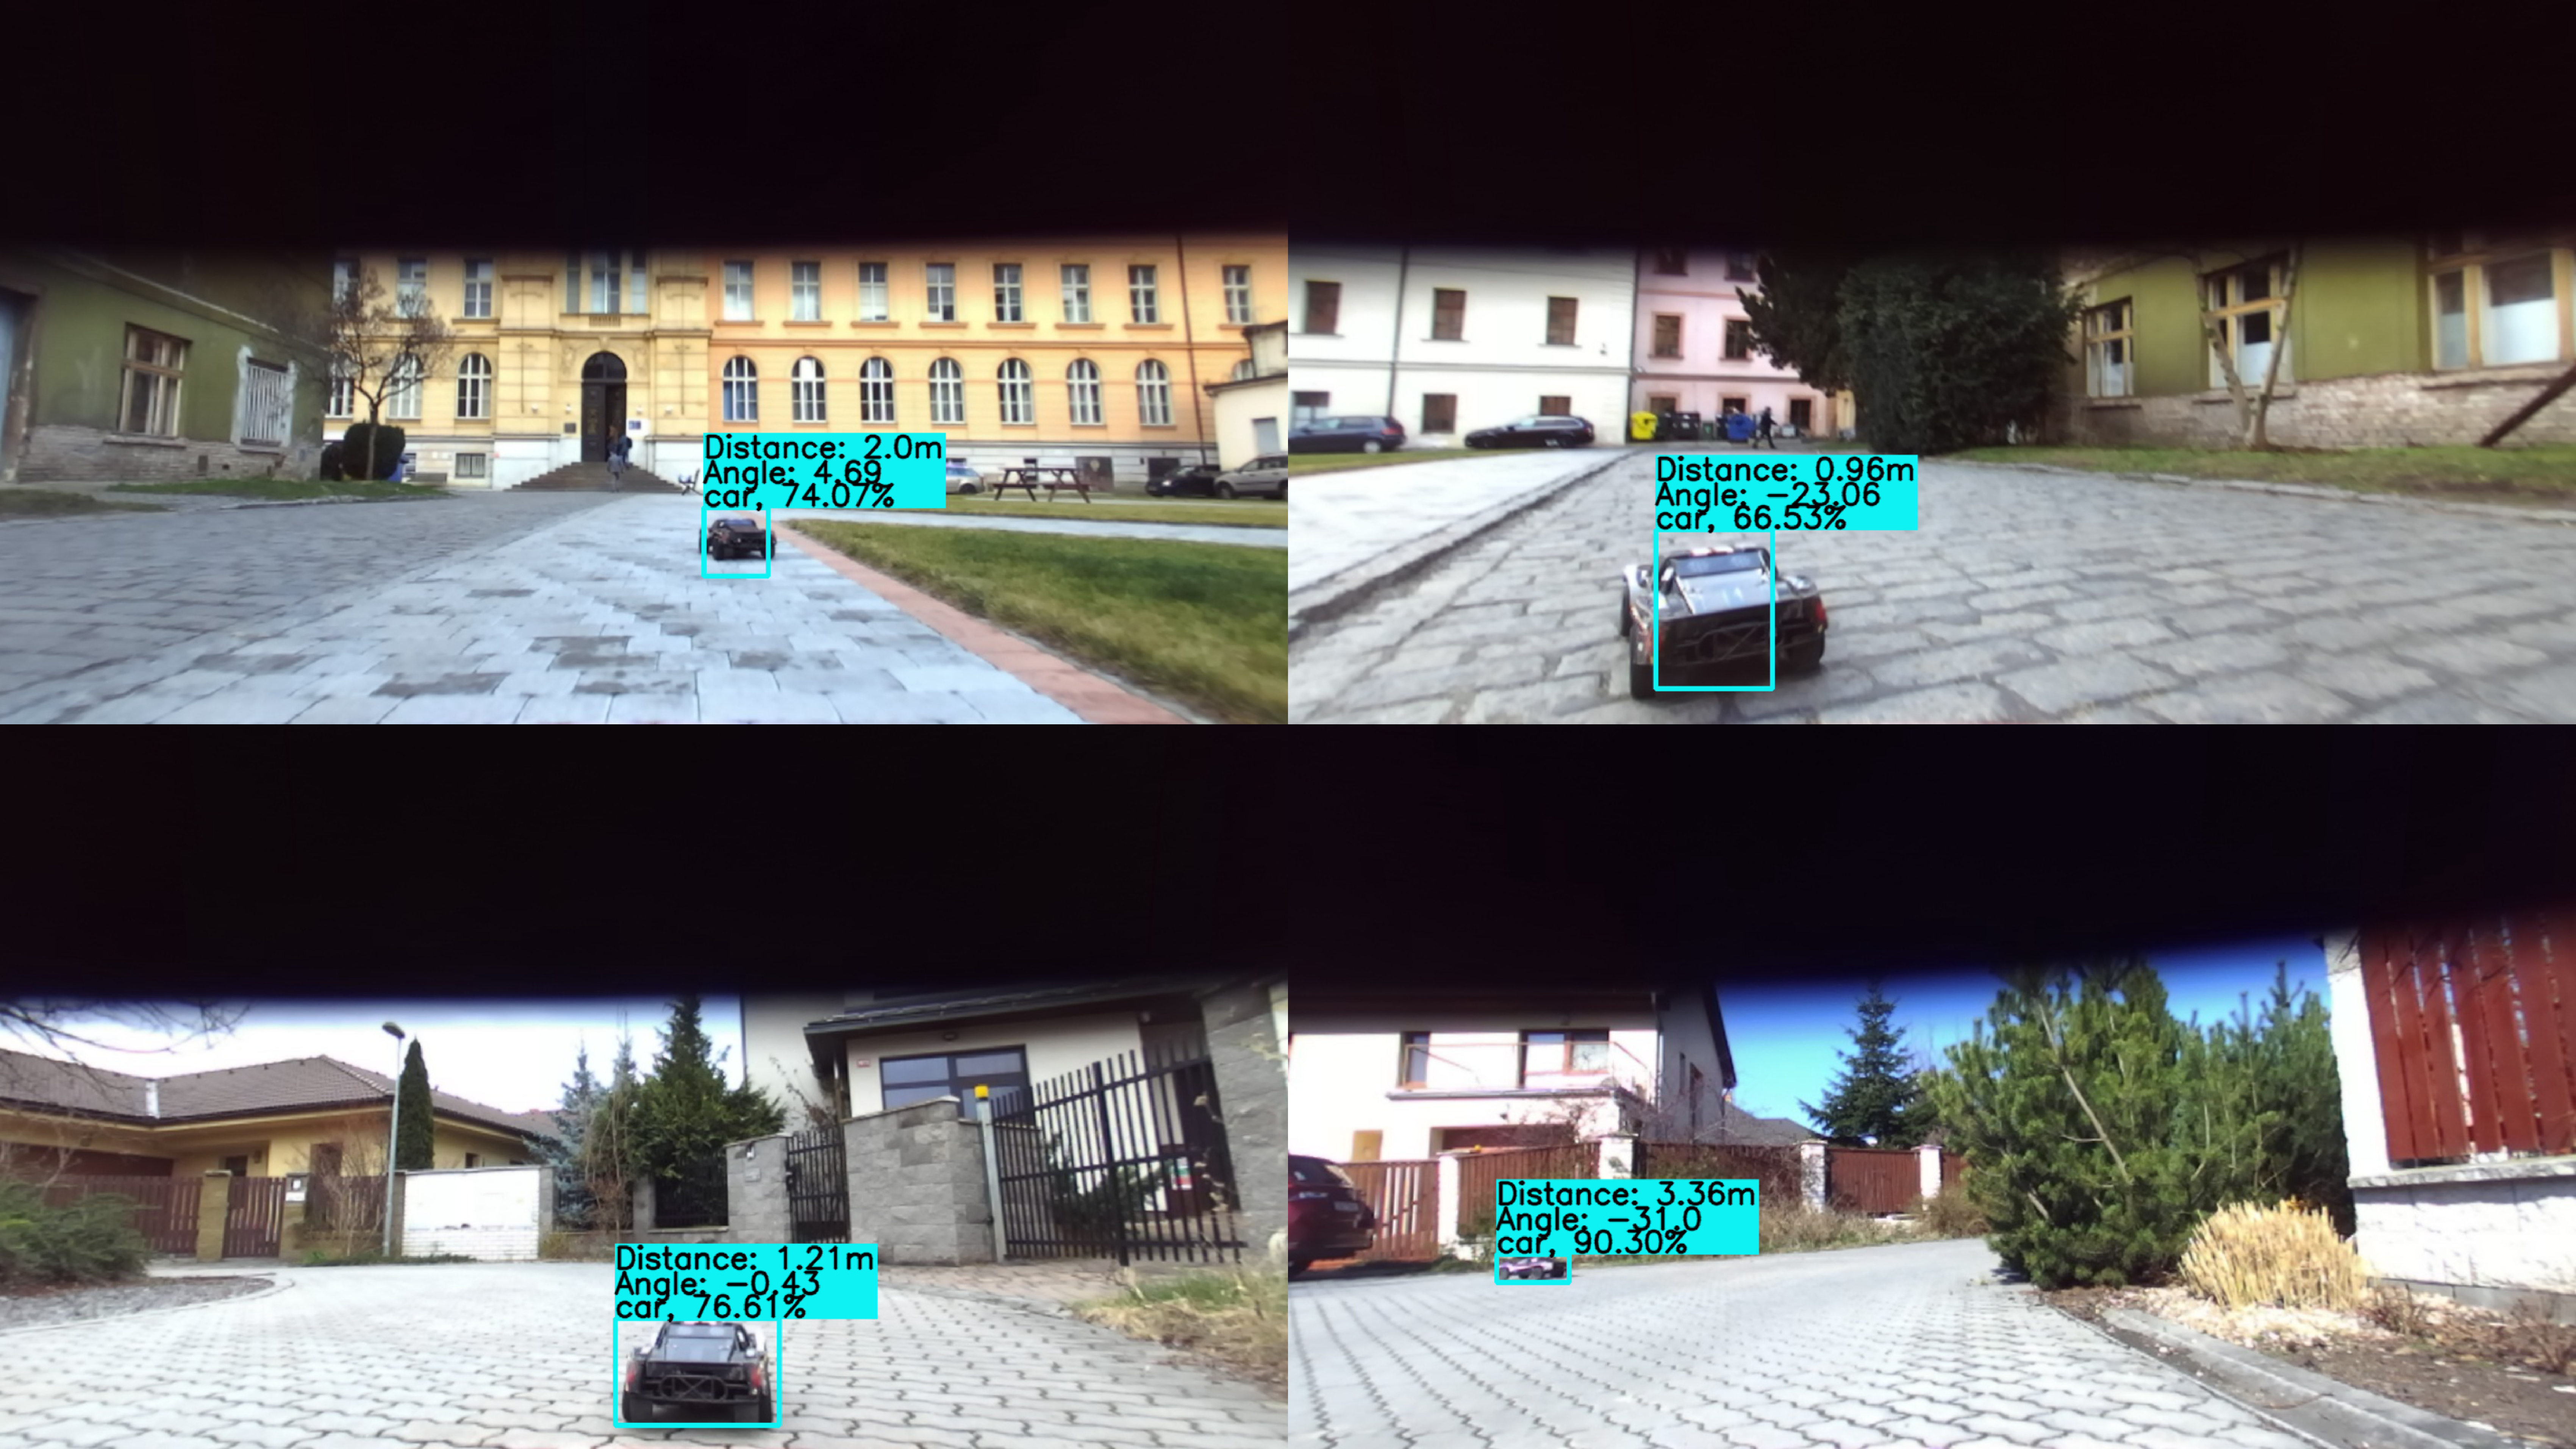
\includegraphics[width=1\textwidth]{images/Collage_detection(1).pdf}
    
    \caption{Detection, distance and angle estimation performed on images from the RC car camera. The images are part of the collected dataset}\label{f:detection_images}
\end{figure}

\section{Simulation}
\subsection{CARLA Environment}
All the simulation experiments were performed in CARLA -- an open-source simulator for autonomous driving research \cite{CARLA}. The experiments were done in a CARLA version 0.9.8. It has a wide selection of sensors including camera, segmentation camera, LIDAR on so on. It provides multiple maps with urban layout. The users can control weather, as well as many different actors (vehicles, pedestrians) at the same time. \par




\subsection{Experiment Setup}
In our work, we have chosen Tesla Model 3 as the chased car and Jeep Wrangler Rubicon as the chasing car. Also, all the experiments were performed in a synchronous mode in which the simulation waits for the sensor data to be ready before sending the measurements as well as halts each frame until a control message is received \cite{CARLA}. \par

To perform the experiments we first collected a driving dataset. We used the Tesla Model 3 and drove it around the city. As the car was driven, its location and orientation was recorded at every frame. This way, we have created a database of 20 different drives with varying difficulty (in a sense of chasing the car). We used this database to evaluate the autonomous driving system. In the following experiments a chasing car was placed 2 meters behind the chased car. Then, we updated every frame the location and orientation of the chased car based on the saved coordinates in the dataset. Meanwhile the chasing vehicle was driven autonomously and trying to maintain desired distance from the pursued car. 




\subsection{Segmentation and Extrapolation Evaluation}
In the first experiment, we compare different versions of the algorithm. We evaluate the algorithm with its full functionality enabled as described in the Method section, we test the same algorithm without using rough image segmentation and finally evaluate the algorithm without image segmentation, and distance and angle extrapolation. \par


We evaluate these verions on the driving dataset. We divide the dataset in two equal sized sets based on difficulty. The first set contains simple drives in which the car was driven slowly and without sudden turning and braking. Any changes such as turns were slow. The average speed in these drives is TODO\par


On the other hand, the second set aims to test the algorithm to its limits. The drives include sudden braking, fast turns as well as cutting corners. Sometimes even drifts were performed. The average speed in these drives is TODO.


\begin{table}[]
\tabcolsep=0.11cm
\begin{tabular}{l|lllll}
\hline
                                       & Finished & Avg. Completion  & Crashes & MAE  & RMSE   \\ \hline
Full Algorithm                         & 10       & 97.48\% & 0.1     & 9.28 & 118.95 \\
W/o Segmentation                    & 10       & 97.41\%          & 0.1     & 9.26 & 118.82 \\
W/o Segm. and Ex. & 9        & 97.03\%          & 0.11    & 9.34 & 126.20 \\ \hline
\end{tabular}
\caption{Comparison of the different algorithm versions on the easy driving set}
\end{table}

\begin{table}[]
\tabcolsep=0.11cm
\begin{tabular}{l|lllll}
\hline
                                       & Finished & Avg. Completion & Crashes & MAE   & RMSE   \\ \hline
Full Algorithm                         & 4               & \textbf{63.84\%}         & 1.5     & 14.39 & 335    \\
W/o Segmentation                   & 4               & 54.76\%                  & 1.25    & 14.30 & 331.89 \\
W/o Segm. and Ex. & 3               & 53.29\%                  & 1       & 14.49 & 357    \\ \hline
\end{tabular}
\caption{Comparison of the different algorithm versions on the difficult driving set}
\end{table}


\subsection{Detection Recall Experiment}

\section{Real-world Testing}
\subsection{RC Cars Description}
\subsubsection{Chasing RC car}
For the deployment of our autonomous chasing algorithm a sub-scale vehicle platform called Toyota Mini (ToMi) was used %TODO cite. 
The platform is built around a large 1:5 scale RC car "Losi Desert Buggy XL-E 4WD". This electrically powered car has 0.9 x 0.5 meters length and width dimensions with reported maximal speed of up to 80km/h. At the core of the platform is a Raspberry Pi with a Navio-board that generates pulse width modulation signals for the throttle and steering to the servomotor. It is also equipped with a ZED stereo camera for taking color images, NVIDIA Jetson AGX Xavier graphics card for image processing and neural network interference. Finally, it is equipped with SSD to provide additional storage, GPS and IMU. \par
The whole simplified process flow is as follows. First, an image is taken by camera, which then goes to graphics card where it's analyzed by our algorithm. Then, based on the image analysis a steer and throttle values are updated. These values are transmitted from the graphics card to the Raspberry Pi which then sends signal to the servomotor that controls the vehicle.

\subsubsection{Chased RC car}
The RC car used as the chased vehicle is a 1:10 scale "Losi XXX-SCR RTR". This electrically powered car has 0.55 x 0.29 meters length and width dimensions with reported maximal speed of up to 55 km/h.

\begin{figure}[h!]
    \centering
    \subfloat[Inside of the chasing RC car]{{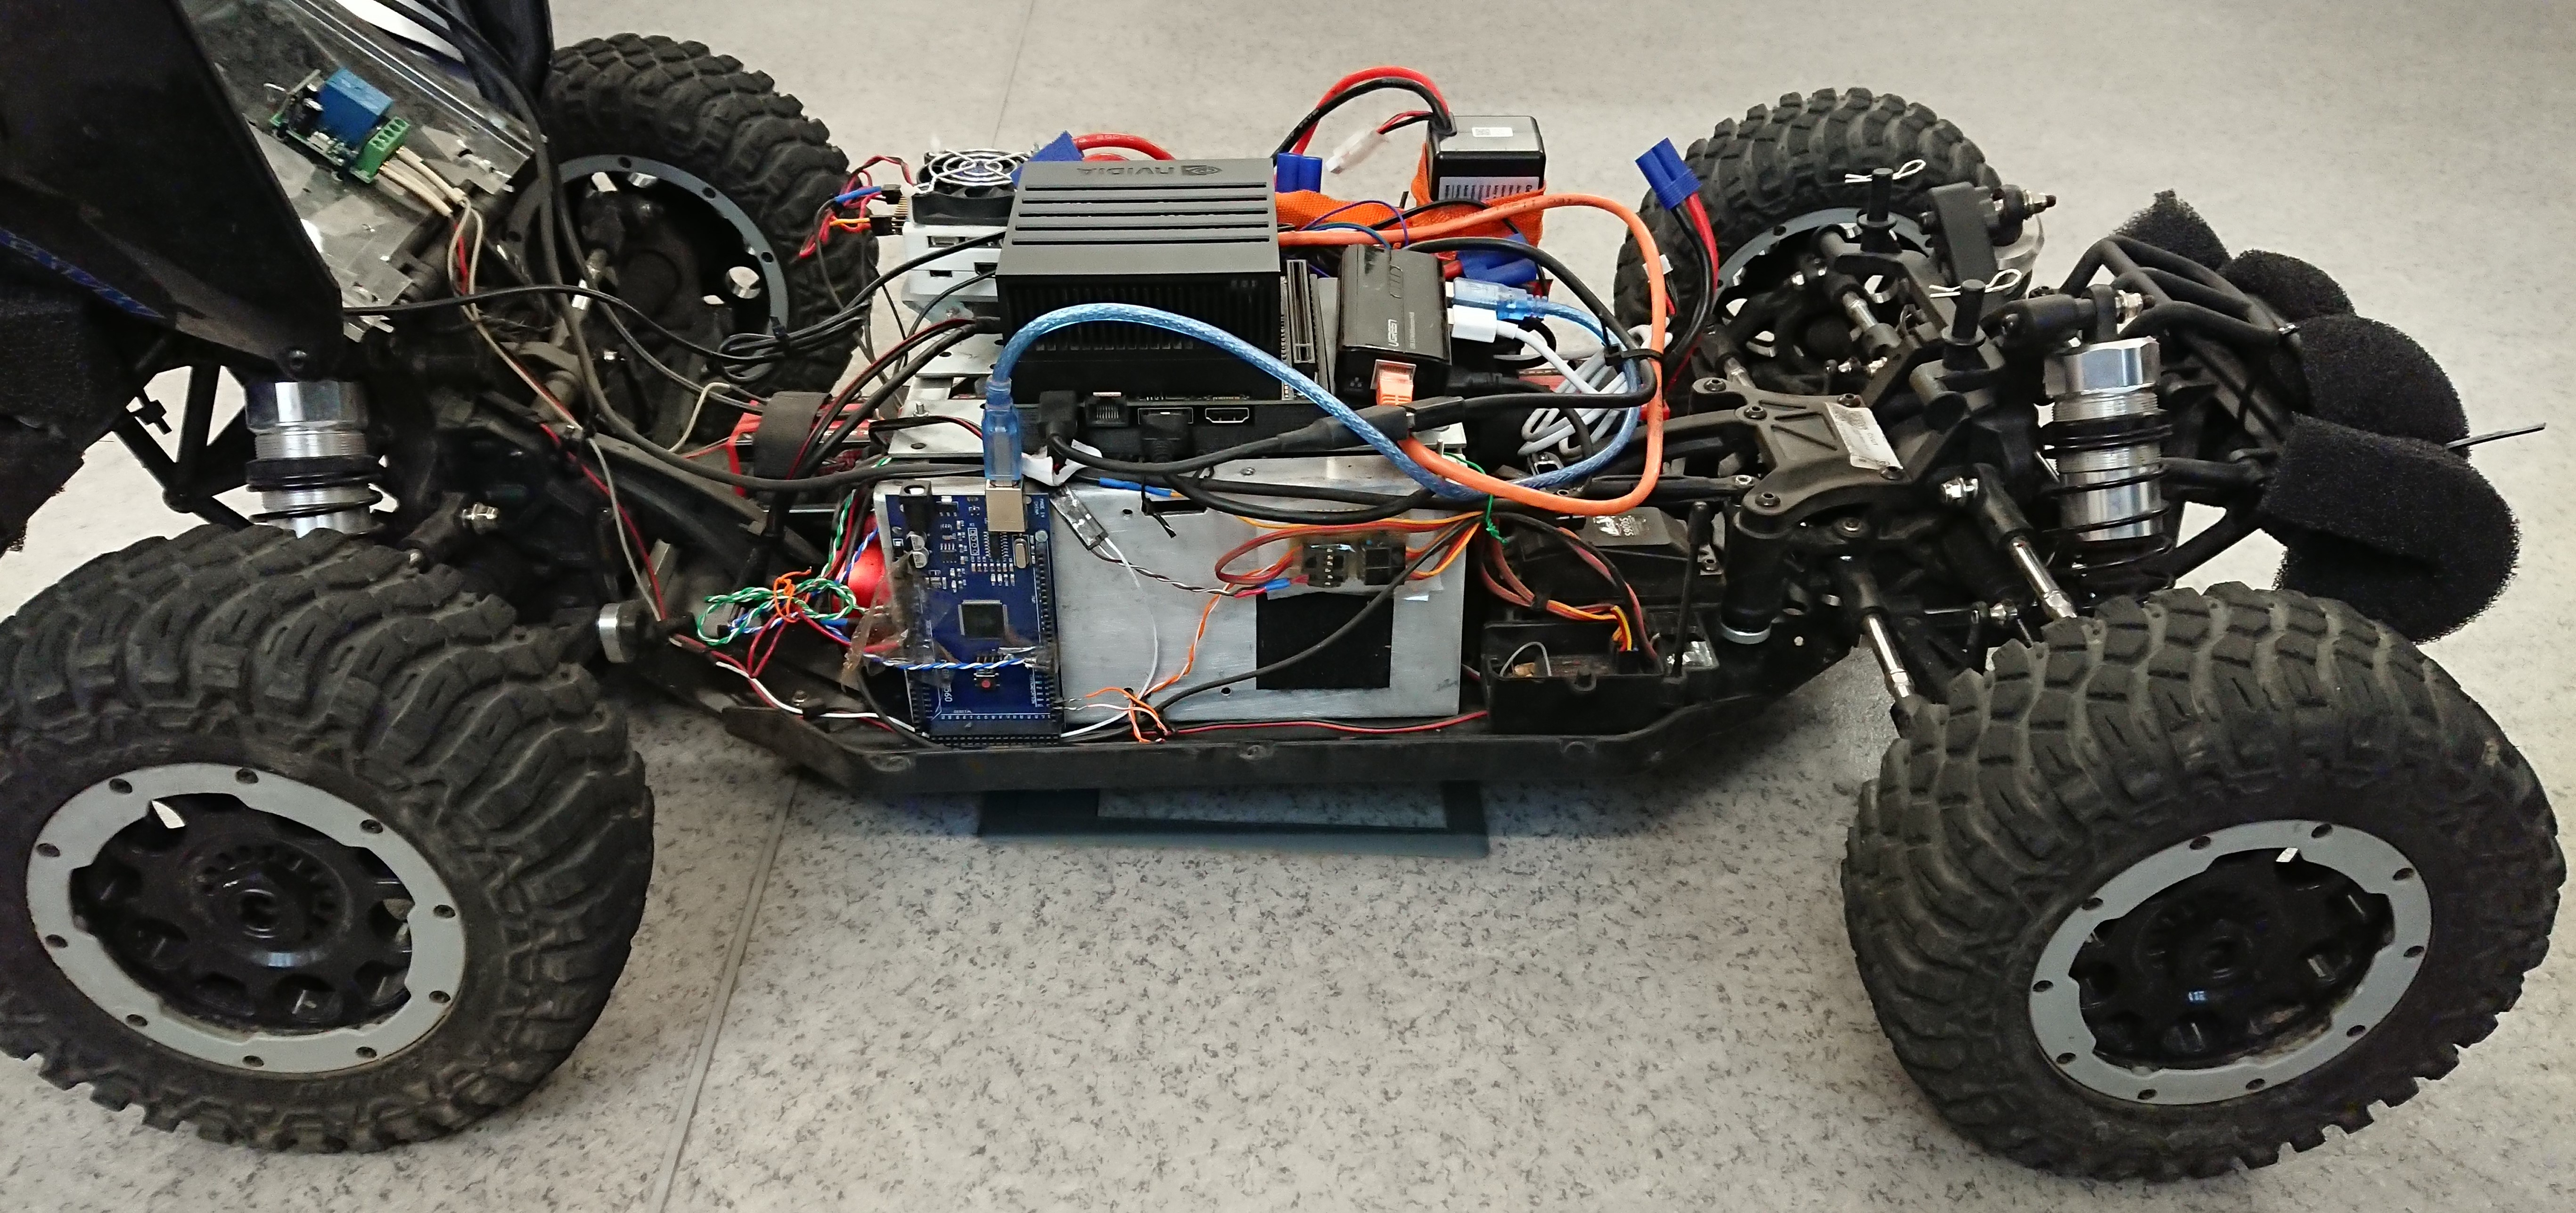
\includegraphics[height=3.7cm]{images/inside.jpg} }}%
    \qquad
    \subfloat[Chasing RC in the back and the chased RC car in the front]{{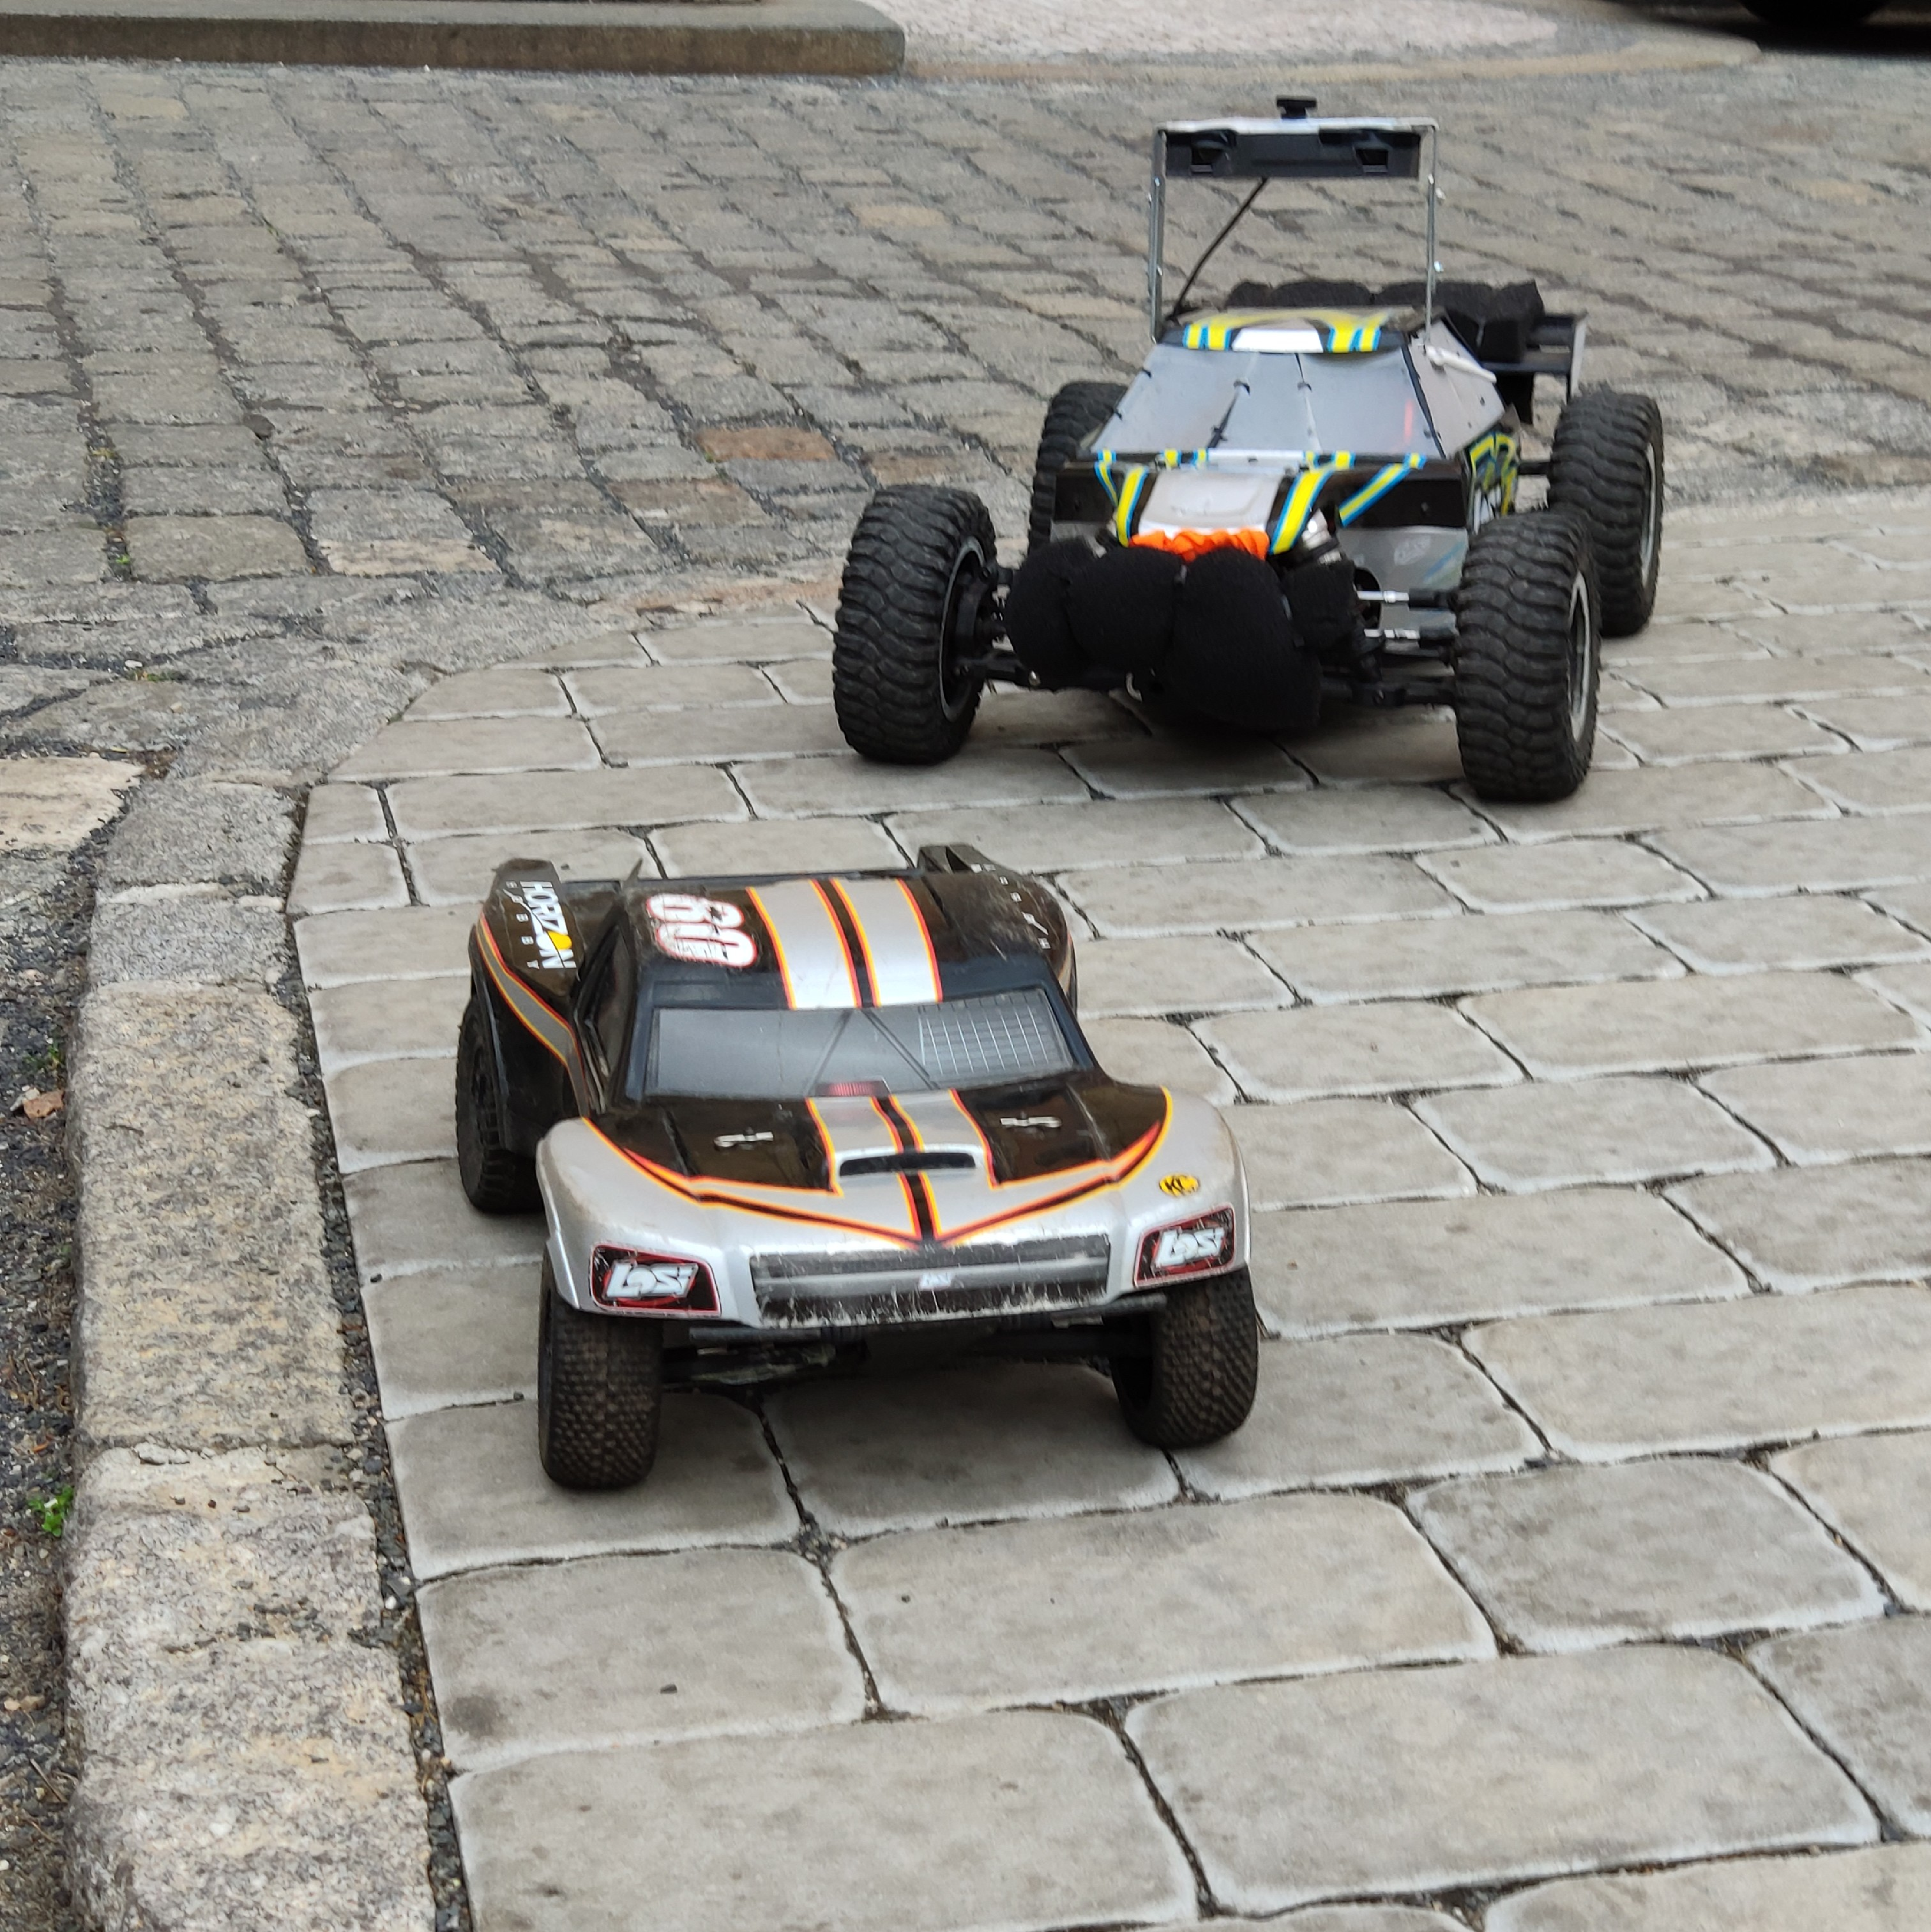
\includegraphics[height=3.7cm]{images/rc_cars.pdf} }}%
    \caption{Hardware inside of the autonomous chasing RC car on the left and both RC cars used for testing on the right}%
    \label{fig:rc_cars}%
\end{figure}

%\begin{figure}[h!]
%\centering
%\begin{subfigure}{.5\textwidth}
%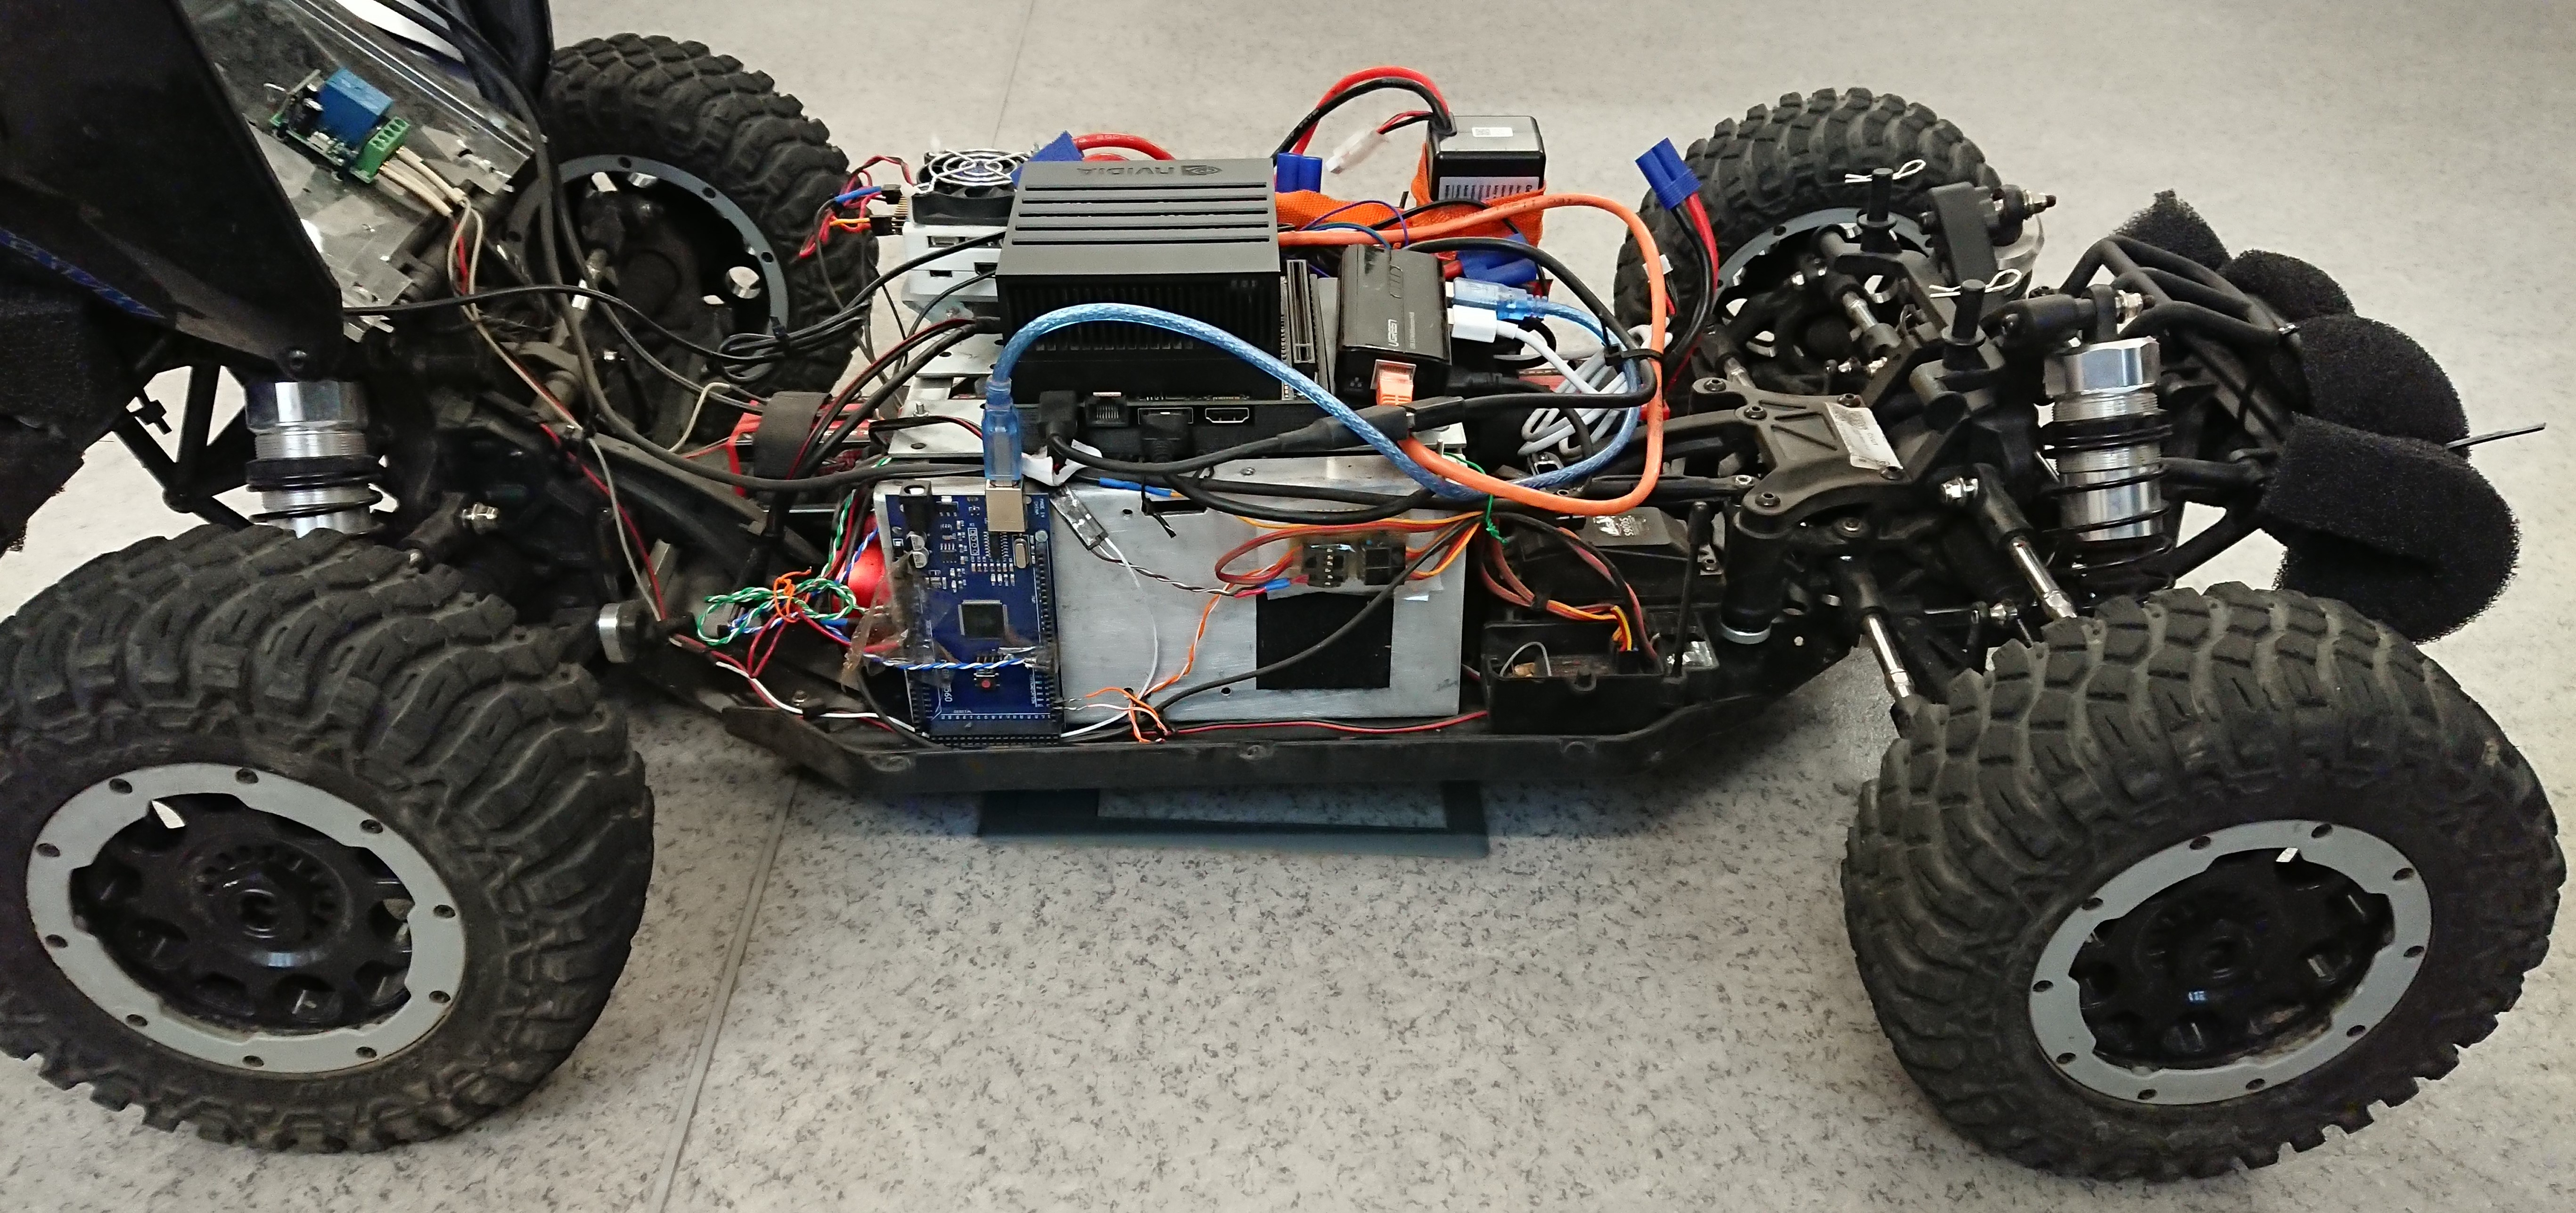
\includegraphics[width=.4\linewidth]{images/inside.jpg}
%\end{subfigure}
%\begin{subfigure}{0.5\textwidth}
%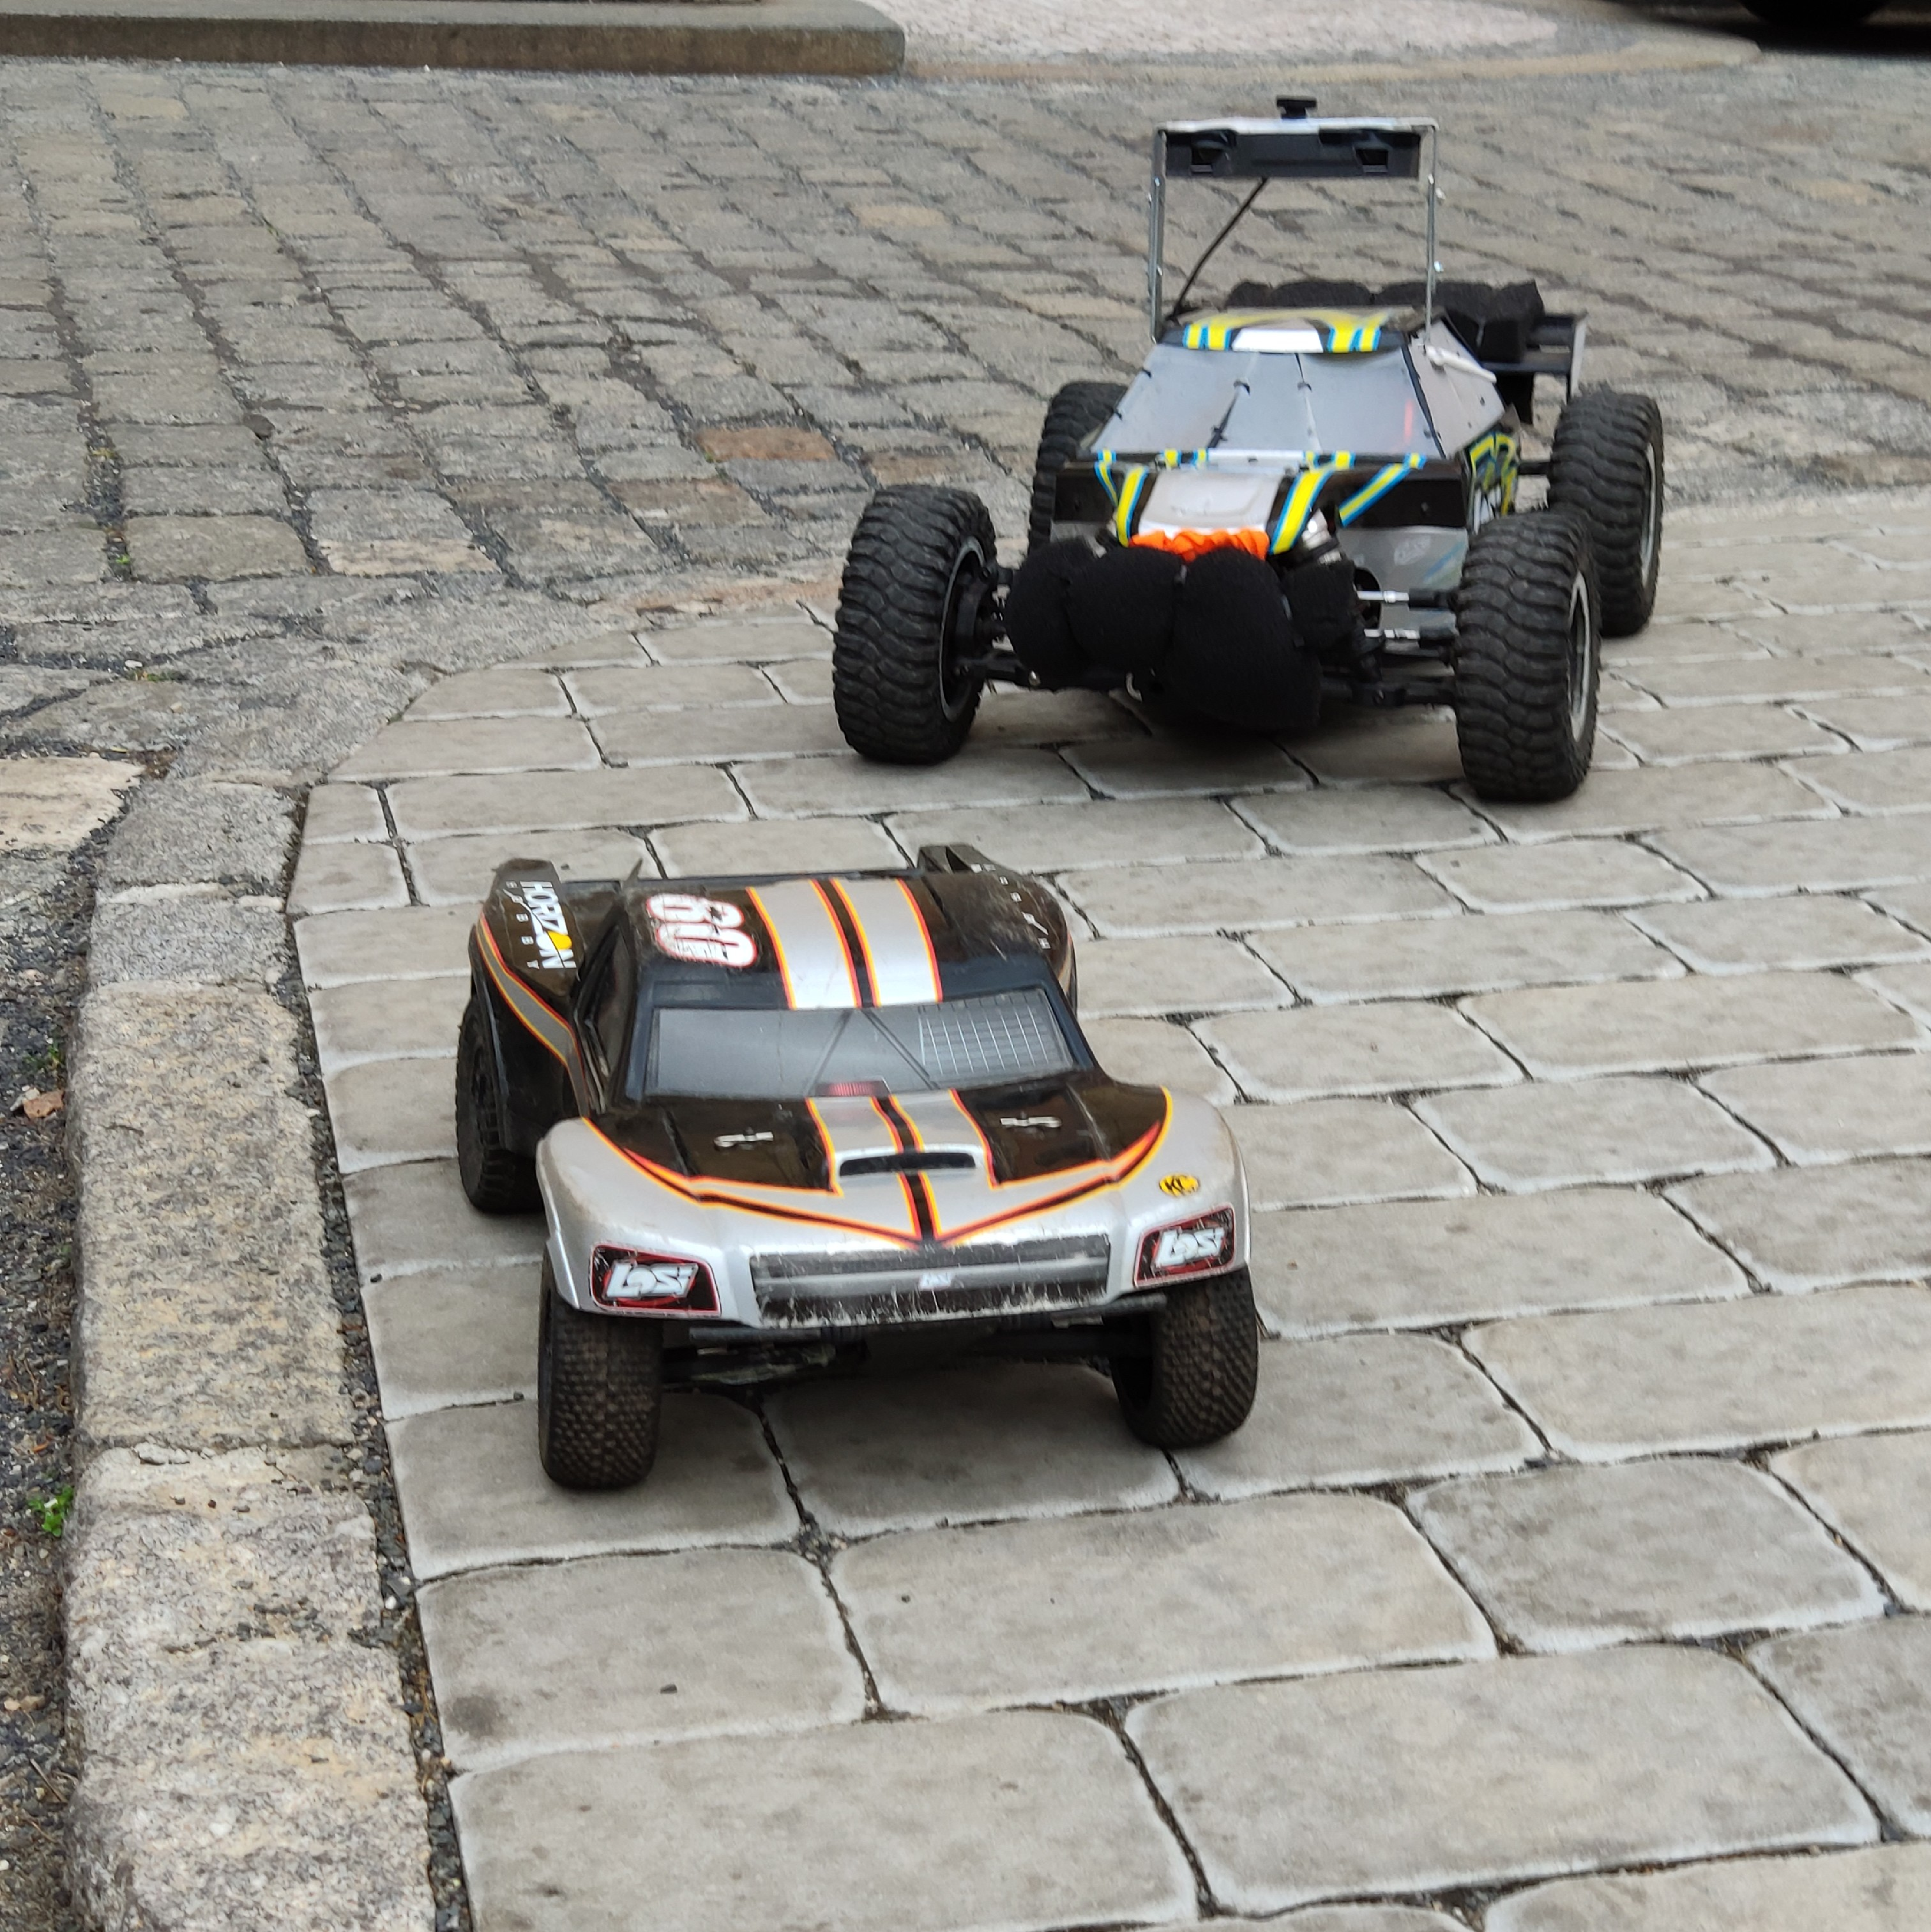
\includegraphics[width=.4\linewidth]{images/rc_cars.pdf}
%\end{subfigure}
%\caption{Both RC cars used for testing. The autonomous chasing car is in the back, while the manually driven car used as the pursued %car is in the front}
%\end{figure}


\subsection{Experiments}



\chapter{Conclusion}

\bibliography{citations}
\bibliographystyle{IEEEtran}

\end{document}

